\makeatletter
\@ifundefined{standalonetrue}{\newif\ifstandalone}{}
\@ifundefined{section}{\standalonetrue}{\standalonefalse}
\makeatother
\ifstandalone
\documentclass{report}

\usepackage{textcase}
%\usepackage{hyperref}
%\hypersetup{breaklinks=true}


% Added packages
\usepackage[usenames]{color}
\usepackage{amsfonts, amsmath, amssymb, graphics}

% NOTE: bibentry MUST appear before the hyperref or build will fail
\usepackage{bibentry}
\nobibliography*
\usepackage[square,sort,comma,numbers]{natbib}
  
\usepackage{float}
\usepackage[
	hidelinks,%
    %hyperindex=true,		% Make numbers of index links as well
   	backref=page, 		% Provide page listing where refs occur in the bibliography
	%breaklinks=true,
    %colorlinks,%
    %citecolor=green,%
    %filecolor=blue,%
    %linkcolor=red,%
    %urlcolor=red, 
]{hyperref}

\usepackage{dsfont}
%%%% USEPACKAGES for MACROS %%%%%
\usepackage{algpseudocode}
\usepackage[chapter]{algorithm}
%\usepackage{caption}
\usepackage{subcaption}
\usepackage{url}

\usepackage{array}
\usepackage{arydshln}
\usepackage{multirow}
\usepackage{multicol}
%\usepackage[section]{placeins}

\usepackage[usenames,dvipsnames]{color}
%\usepackage[english]{babel}
\usepackage{tabularx}
\usepackage{soul}
\usepackage{xparse}
\usepackage{listings}
%\usepackage[normalem]{ulem}



%%%%%%%%%%%%%%%
% Show a list of items "todo" or "done" 
% USAGE: 
% \begin{todolist} 
% 	\todo Something not finished
% 	\done Something finished
% \end{todolist} 
\newenvironment{todolist}{%
  \begin{list}{}{}% whatever you want the list to be
  \let\olditem\item
  \renewcommand\item{\olditem \textcolor{red}{(TODO)}: }
  \newcommand\todo{\olditem \textcolor{red}{(TODO)}: }
   \newcommand\done{\olditem \textcolor{ForestGreen}{(DONE)}: }
}{%
  \end{list}
} 
%%%%%%%%%%%%%%%

%%%%%%%%%%%%%%%
% Show a Author's Note
% USAGE: 
% \incomplete[Optional footnote message to further clarify note]{The text which is currently not finished}
\DeclareDocumentCommand \incomplete{ o m }
{%
\IfNoValueTF {#1}
{\textcolor{red}{Incomplete: \ul{#2}}} 
{\textcolor{red}{Incomplete: \ul{#2}}\footnote{Comment: #1}}%
}
%%%%%%%%%%%%%%%



%%%%%%%%%%%%%%%
% Show a Author's Note
% USAGE: 
% \authnote[Optional footnote message to further clarify note]{The note to your readers}
\DeclareDocumentCommand \authnote { o m }
{%
\IfNoValueTF {#1}
{\textcolor{blue}{Author's Note: \ul{#2}}} 
{\textcolor{blue}{Author's Note: \ul{#2}}\footnote{Comment: #1}}%
}
%%%%%%%%%%%%%%%



%%%%%%%%%%%%%%%
% Strike out text that doesn't belong in the paper
% USAGE: 
% \strike[Optional footnote to state why it doesn't belong]{Text to strike out}
\DeclareDocumentCommand \strike { o m }
{%
\setstcolor{Red}
\IfNoValueTF {#1}
{\textcolor{Gray}{\st{#2}}} 
{\textcolor{Gray}{\st{#2}}\footnote{Comment: #1}}%
}
%%%%%%%%%%%%%%%

\definecolor{light-gray}{gray}{0.95}

\newcommand{\cbox}[3]{
\ \\
\fcolorbox{#1}{#2}{
\parbox{\textwidth}{
#3
}
}
}

% Setup an environment similar to verbatim but which will highlight any bash commands we have
\lstnewenvironment{unixcmds}[0]
{
%\lstset{language=bash,frame=shadowbox,rulesepcolor=\color{blue}}
\lstset{ %
language=sh,		% Language
basicstyle=\ttfamily,
backgroundcolor=\color{light-gray}, 
rulecolor=\color{blue},
%frame=tb, 
columns=fullflexible,
%framexrightmargin=-.2\textwidth,
linewidth=0.8\textwidth,
breaklines=true,
%prebreak=/, 
  prebreak = \raisebox{0ex}[0ex][0ex]{\ensuremath{\hookleftarrow}},
%basicstyle=\footnotesize,       % the size of the fonts that are used for the code
%numbers=left,                   % where to put the line-numbers
%numberstyle=\footnotesize,      % the size of the fonts that are used for the line-numbers
%stepnumber=2,                   % the step between two line-numbers. If it's 1 each line 
                                % will be numbered
%numbersep=5pt,                  % how far the line-numbers are from the code
showspaces=false,               % show spaces adding particular underscores
showstringspaces=false,         % underline spaces within strings
showtabs=false,                 % show tabs within strings adding particular underscores
frame=single,	                % adds a frame around the code
tabsize=2,	                % sets default tabsize to 2 spaces
captionpos=b,                   % sets the caption-position to bottom
breakatwhitespace=false,        % sets if automatic breaks should only happen at whitespace
}
} { }

% Setup an environment similar to verbatim but which will highlight any bash commands we have
\lstnewenvironment{cppcode}[1]
{
%\lstset{language=bash,frame=shadowbox,rulesepcolor=\color{blue}}
\lstset{ %
	backgroundcolor=\color{light-gray}, 
	rulecolor=\color[rgb]{0.133,0.545,0.133},
	tabsize=4,
	language=[GNU]C++,
%	basicstyle=\ttfamily,
        basicstyle=\scriptsize,
        upquote=true,
        aboveskip={1.5\baselineskip},
        columns=fullflexible,
        %framexrightmargin=-.1\textwidth,
       %framexleftmargin=6mm,
        showstringspaces=false,
        extendedchars=true,
        breaklines=true,
        prebreak = \raisebox{0ex}[0ex][0ex]{\ensuremath{\hookleftarrow}},
        frame=single,
        showtabs=false,
        showspaces=false,
        showstringspaces=false,
        numbers=left,                   % where to put the line-numbers
	numberstyle=\footnotesize,      % the size of the fonts that are used for the line-numbers
	stepnumber=4,                   % the step between two line-numbers. If it's 1 each line 
                                % will be numbered
	firstnumber=#1,
         numbersep=5pt,                  % how far the line-numbers are from the code
        identifierstyle=\ttfamily,
        keywordstyle=\color[rgb]{0,0,1},
        commentstyle=\color[rgb]{0.133,0.545,0.133},
        stringstyle=\color[rgb]{0.627,0.126,0.941},
}
} { }

% Setup an environment similar to verbatim but which will highlight any bash commands we have
\lstnewenvironment{mcode}[1]
{
\lstset{ %
	backgroundcolor=\color{light-gray}, 
	rulecolor=\color[rgb]{0.133,0.545,0.133},
	tabsize=4,
	language=Matlab,
%	basicstyle=\ttfamily,
        basicstyle=\scriptsize,
        upquote=true,
        aboveskip={1.5\baselineskip},
        columns=fullflexible,
        %framexrightmargin=-.1\textwidth,
       %framexleftmargin=6mm,
        showstringspaces=false,
        extendedchars=true,
        breaklines=true,
        prebreak = \raisebox{0ex}[0ex][0ex]{\ensuremath{\hookleftarrow}},
        frame=single,
        showtabs=false,
        showspaces=false,
        showstringspaces=false,
        numbers=left,                   % where to put the line-numbers
	numberstyle=\footnotesize,      % the size of the fonts that are used for the line-numbers
	stepnumber=4,                   % the step between two line-numbers. If it's 1 each line 
                                % will be numbered
	firstnumber=#1,
         numbersep=5pt,                  % how far the line-numbers are from the code
        identifierstyle=\ttfamily,
        keywordstyle=\color[rgb]{0,0,1},
        commentstyle=\color[rgb]{0.133,0.545,0.133},
        stringstyle=\color[rgb]{0.627,0.126,0.941},
}
} { }

\newcommand{\inputmcode}[1]{%
\lstset{ %
	backgroundcolor=\color{light-gray},  %
	rulecolor=\color[rgb]{0.133,0.545,0.133}, %
	tabsize=4, %
	language=Matlab, %
%	basicstyle=\ttfamily,
        basicstyle=\scriptsize, %
        %        upquote=true,
        aboveskip={1.5\baselineskip}, %
        columns=fullflexible, %
        %framexrightmargin=-.1\textwidth,
       %framexleftmargin=6mm,
        showstringspaces=false, %
        extendedchars=true, %
        breaklines=true, %
        prebreak = \raisebox{0ex}[0ex][0ex]{\ensuremath{\hookleftarrow}}, %
        frame=single, %
        showtabs=false, %
        showspaces=false, %
        showstringspaces=false,%
        numbers=left,                   % where to put the line-numbers
	numberstyle=\footnotesize,      % the size of the fonts that are used for the line-numbers
	stepnumber=4,                   % the step between two line-numbers. If it's 1 each line 
                                % will be numbered
         numbersep=5pt,                  % how far the line-numbers are from the code
        identifierstyle=\ttfamily, %
        keywordstyle=\color[rgb]{0,0,1}, %
        commentstyle=\color[rgb]{0.133,0.545,0.133}, %
        stringstyle=\color[rgb]{0.627,0.126,0.941} %
}
\lstinputlisting{#1}%
}

%\lstset{ %
%	backgroundcolor=\color{light-gray}, 
%	rulecolor=\color[rgb]{0.133,0.545,0.133},
%	tabsize=4,
%	language=Matlab,
%%	basicstyle=\ttfamily,
%        basicstyle=\scriptsize,
%        upquote=true,
%        aboveskip={1.5\baselineskip},
%        columns=fullflexible,
%        %framexrightmargin=-.1\textwidth,
%       %framexleftmargin=6mm,
%        showstringspaces=false,
%        extendedchars=true,
%        breaklines=true,
%        prebreak = \raisebox{0ex}[0ex][0ex]{\ensuremath{\hookleftarrow}},
%        frame=single,
%        showtabs=false,
%        showspaces=false,
%        showstringspaces=false,
%        numbers=left,                   % where to put the line-numbers
%	numberstyle=\footnotesize,      % the size of the fonts that are used for the line-numbers
%	stepnumber=4,                   % the step between two line-numbers. If it's 1 each line 
%                                % will be numbered
%	firstnumber=#1,
%         numbersep=5pt,                  % how far the line-numbers are from the code
%        identifierstyle=\ttfamily,
%        keywordstyle=\color[rgb]{0,0,1},
%        commentstyle=\color[rgb]{0.133,0.545,0.133},
%        stringstyle=\color[rgb]{0.627,0.126,0.941},
%}


\newcommand{\Laplacian}[1]{\nabla^2 #1}

% set of all nodes received and contained on GPU
\newcommand{\setAllNodes}[0]{\mathcal{G}}
% set of stencil centers on GPU
\newcommand{\setCenters}[0]{\mathcal{Q}}
% set of stencil centers with nodes in \setDepend
\newcommand{\setBoundary}[0]{\mathcal{B}}
% set of nodes received by other GPUs
\newcommand{\setDepend}[0]{\mathcal{R}}
% set of nodes sent to other GPUs
\newcommand{\setProvide}[0]{\mathcal{O}}


\newcommand{\toprule}[0]{\hline}
\newcommand{\midrule}[0]{\hline\hline}
\newcommand{\bottomrule}[0]{\hline}

\newcolumntype{C}{>{\centering\arraybackslash}b{1in}}
\newcolumntype{L}{>{\flushleft\arraybackslash}b{1.5in}}
\newcolumntype{R}{>{\flushright\arraybackslash}b{1.5in}}
\newcolumntype{D}{>{\flushright\arraybackslash}b{2.0in}}
\newcolumntype{E}{>{\flushright\arraybackslash}b{1.0in}}

\DeclareSymbolFont{AMSb}{U}{msb}{m}{n}
\DeclareMathSymbol{\N}{\mathbin}{AMSb}{"4E}
\DeclareMathSymbol{\Z}{\mathbin}{AMSb}{"5A}
\DeclareMathSymbol{\R}{\mathbin}{AMSb}{"52}
\DeclareMathSymbol{\Q}{\mathbin}{AMSb}{"51}
\DeclareMathSymbol{\PP}{\mathbin}{AMSb}{"50}
\DeclareMathSymbol{\I}{\mathbin}{AMSb}{"49}
%\DeclareMathSymbol{\C}{\mathbin}{AMSb}{"43}

%%%%%% VECTOR NORM: %%%%%%%
\newcommand{\vectornorm}[1]{\left|\left|#1\right|\right|}
\newcommand{\vnorm}[1]{\left|\left|#1\right|\right|}
\newcommand{\by}[0]{\times}
\newcommand{\vect}[1]{\mathbf{#1}}
%\newcommand{\mat}[1]{\mathbf{#1}} 

%\renewcommand{\vec}[1]{ \textbf{#1} }
%%%%%%%%%%%%%%%%%%%%%%

%%%%%%% THM, COR, DEF %%%%%%%
%\newtheorem{theorem}{Theorem}[section]
%\newtheorem{lemma}[theorem]{Lemma}
%\newtheorem{proposition}[theorem]{Proposition}
%\newtheorem{corollary}[theorem]{Corollary}
%\newenvironment{proof}[1][Proof]{\begin{trivlist}
%\item[\hskip \labelsep {\bfseries #1}]}{\end{trivlist}}
%\newenvironment{definition}[1][Definition]{\begin{trivlist}
%\item[\hskip \labelsep {\bfseries #1}]}{\end{trivlist}}
%\newenvironment{example}[1][Example]{\begin{trivlist}
%\item[\hskip \labelsep {\bfseries #1}]}{\end{trivlist}}
%\newenvironment{remark}[1][Remark]{\begin{trivlist}
%\item[\hskip \labelsep {\bfseries #1}]}{\end{trivlist}}
%\newcommand{\qed}{\nobreak \ifvmode \relax \else
%      \ifdim\lastskip<1.5em \hskip-\lastskip
%      \hskip1.5em plus0em minus0.5em \fi \nobreak
%      \vrule height0.75em width0.5em depth0.25em\fi}
%%%%%%%%%%%%%%%%%%%%%%

%
%\usepackage[algochapter]{algorithm2e}
%\usepackage[usenames]{color}
% colors to show the corrections
\newcommand{\red}[1]{\textbf{\textcolor{red}{#1}}}
\newcommand{\blue}[1]{\textbf{\textcolor{blue}{#1}}}
\newcommand{\cyan}[1]{\textbf{\textcolor{cyan}{#1}}}
\newcommand{\green}[1]{\textbf{\textcolor{green}{#1}}}
\newcommand{\magenta}[1]{\textbf{\textcolor{magenta}{#1}}}
\newcommand{\orange}[1]{\textbf{\textcolor{orange}{#1}}}
%%%%%%%%%% DK DK
% comments between authors
\newcommand{\toall}[1]{\textbf{\green{@@@ All: #1 @@@}}}
\newcommand{\toevan}[1]{\textbf{\red{*** Evan: #1 ***}}}
%\newcommand{\toevan}[1]{}  % USE FOR FINAL VERSION
\newcommand{\toe}[1]{\textbf{\red{*** Evan: #1 ***}}}
\newcommand{\tog}[1]{\textbf{\blue{*** Gordon: #1 ***}}}
%\newcommand{\togordon}[1]{\textbf{\blue{*** Gordon: #1 ***}}}
\renewcommand{\ge}[3]{{\textcolor{blue}{*** \textbf{Gordon:}\strike{#1} #2 ***}}\red{(#3)}}
\renewcommand{\ge}[3]{{\textcolor{blue}{#2}}}
\renewcommand{\ge}[3]{{\textcolor{Red}{#2}}}
\newcommand{\eb}[3]{{\textcolor{Red}{*** \textbf{Evan:}\strike{#1} #2 ***}}\red{(#3)}}
\renewcommand{\eb}[3]{{{\textcolor{Red}{#2}}}}
%\def\ge#1#2#3{}{\textbf{\blue{*** Gordon: #2 ***}}}{(#3)}
\newcommand{\gee}[1]{{\bf{\blue{{\em #1}}}}}
\newcommand{\old}[1]{}
\newcommand{\del}[1]{***#1*** }



% \DeclareMathOperator{\Sample}{Sample}
%\let\vaccent=\v % rename builtin command \v{} to \vaccent{}
%\renewcommand{\vec}[1]{\ensuremath{\mathbf{#1}}} % for vectors
\newcommand{\gv}[1]{\ensuremath{\mbox{\boldmath$ #1 $}}} 
% for vectors of Greek letters
\newcommand{\uv}[1]{\ensuremath{\mathbf{\hat{#1}}}} % for unit vector
\newcommand{\abs}[1]{\left| #1 \right|} % for absolute value
\newcommand{\avg}[1]{\left< #1 \right>} % for average
\let\underdot=\d % rename builtin command \d{} to \underdot{}
\renewcommand{\d}[2]{\frac{d #1}{d #2}} % for derivatives
\newcommand{\dd}[2]{\frac{d^2 #1}{d #2^2}} % for double derivatives
\newcommand{\pd}[2]{\frac{\partial #1}{\partial #2}} 
% for partial derivatives
\newcommand{\pdd}[2]{\frac{\partial^2 #1}{\partial #2^2}} 
\newcommand{\pdda}[3]{\frac{\partial^2 #1}{\partial #2 \partial #3}} 
% for double partial derivatives
\newcommand{\pdc}[3]{\left( \frac{\partial #1}{\partial #2}
 \right)_{#3}} % for thermodynamic partial derivatives
\newcommand{\ket}[1]{\left| #1 \right>} % for Dirac bras
\newcommand{\bra}[1]{\left< #1 \right|} % for Dirac kets
\newcommand{\braket}[2]{\left< #1 \vphantom{#2} \right|
 \left. #2 \vphantom{#1} \right>} % for Dirac brackets
\newcommand{\matrixel}[3]{\left< #1 \vphantom{#2#3} \right|
 #2 \left| #3 \vphantom{#1#2} \right>} % for Dirac matrix elements
\newcommand{\grad}[1]{\gv{\nabla} #1} % for gradient
\let\divsymb=\div % rename builtin command \div to \divsymb
\renewcommand{\div}[1]{\gv{\nabla} \cdot #1} % for divergence
\newcommand{\curl}[1]{\gv{\nabla} \times #1} % for curl
\let\baraccent=\= % rename builtin command \= to \baraccent
\renewcommand{\=}[1]{\stackrel{#1}{=}} % for putting numbers above =
\newcommand{\diffop}[1]{\mathcal{L}#1}
\newcommand{\boundop}[1]{\mathcal{B}#1}
\newcommand{\rvec}[0]{{\bf r}}

\newcommand{\Interior}[0]{\Omega}
\newcommand{\domain}[0]{\Omega}
%\newcommand{\Boundary}[0]{\partial \Omega}
\newcommand{\Boundary}[0]{\Gamma}

\newcommand{\on}[1]{\hskip1.5em \textrm{ on } #1}

\newcommand{\gemm}{\texttt{GEMM}}
\newcommand{\trmm}{\texttt{TRMM}}
\newcommand{\gesvd}{\texttt{GESVD}}
\newcommand{\geqrf}{\texttt{GEQRF}}


\newcommand{\minitab}[2][l]{\begin{tabular}{#1}#2\end{tabular}}
\newcommand{\comm}[1]{\textcolor{red}{\textit{#1}}}

\newcommand{\nfrac}[2]{
\nicefrac{#1}{#2}
%\frac{#1}{#2}
}

\usepackage{xparse}
\usepackage{soul}


%%%%%%%%%%%%%%%
% Show a Author's Note
% USAGE: 
% \incomplete[Optional footnote message to further clarify note]{The text which is currently not finished}
\DeclareDocumentCommand \incomplete{ o m }
{%
\IfNoValueTF {#1}
{\textcolor{red}{Incomplete: \ul{#2}}} 
{\textcolor{red}{Incomplete: \ul{#2}}\footnote{Comment: #1}}%
}
%%%%%%%%%%%%%%%



%%%%%%%%%%%%%%%
% Show a Author's Note
% USAGE: 
% \authnote[Optional footnote message to further clarify note]{The note to your readers}
\DeclareDocumentCommand \authnote { o m }
{%
\IfNoValueTF {#1}
{\textcolor{blue}{Author's Note: \ul{#2}}} 
{\textcolor{blue}{Author's Note: \ul{#2}}\footnote{Comment: #1}}%
}
%%%%%%%%%%%%%%%



%%%%%%%%%%%%%%%
% Strike out text that doesn't belong in the paper
% USAGE: 
% \strike[Optional footnote to state why it doesn't belong]{Text to strike out}
\DeclareDocumentCommand \strike { o m }
{%
\setstcolor{red}
\IfNoValueTF {#1}
{\textcolor{Gray}{\st{#2}}} 
{\textcolor{Gray}{\st{#2}}\footnote{Comment: #1}}%
}
%%%%%%%%%%%%%%%



%
% colors to show the corrections
\newcommand{\red}[1]{\textbf{\textcolor{red}{#1}}}
\newcommand{\blue}[1]{\textbf{\textcolor{blue}{#1}}}
\newcommand{\cyan}[1]{\textbf{\textcolor{cyan}{#1}}}
\newcommand{\green}[1]{\textbf{\textcolor{green}{#1}}}
\newcommand{\magenta}[1]{\textbf{\textcolor{magenta}{#1}}}
\newcommand{\orange}[1]{\textbf{\textcolor{orange}{#1}}}
%%%%%%%%%% DK DK
% comments between authors
\newcommand{\toall}[1]{\textbf{\green{@@@ All: #1 @@@}}}
\newcommand{\toevan}[1]{\textbf{\red{*** Evan: #1 ***}}}
%\newcommand{\toevan}[1]{}  % USE FOR FINAL VERSION
\newcommand{\toe}[1]{\textbf{\red{*** Evan: #1 ***}}}
\newcommand{\tog}[1]{\textbf{\blue{*** Gordon: #1 ***}}}
%\newcommand{\togordon}[1]{\textbf{\blue{*** Gordon: #1 ***}}}
\renewcommand{\ge}[3]{{\textcolor{blue}{*** \textbf{Gordon:}\strike{#1} #2 ***}}\red{(#3)}}
\renewcommand{\ge}[3]{{\textcolor{blue}{#2}}}
\renewcommand{\ge}[3]{{\textcolor{red}{#2}}}
\newcommand{\eb}[3]{{\textcolor{red}{*** \textbf{Evan:}\strike{#1} #2 ***}}\red{(#3)}}
\renewcommand{\eb}[3]{{{\textcolor{red}{#2}}}}
%\def\ge#1#2#3{}{\textbf{\blue{*** Gordon: #2 ***}}}{(#3)}
\newcommand{\gee}[1]{{\bf{\blue{{\em #1}}}}}
\newcommand{\old}[1]{}
\newcommand{\del}[1]{***#1*** }



% Rename  this file          misc_mac.tex
%----------------------------------------------------------------------
%%%%%%%%%%%%%%%%%%%%%%%%%%%%%%%%%%%%%%%%%%%%%%%%%%%%%%%%%%%%%%%%%%%%%%%%%%%%%%%
%
%	Math Symbols   Math Symbols   Math Symbols   Math Symbols   
%
%%%%%%%%%%%%%%%%%%%%%%%%%%%%%%%%%%%%%%%%%%%%%%%%%%%%%%%%%%%%%%%%%%%%%%%%%%%%%%%
\def\pmb#1{\setbox0=\hbox{$#1$}%
	\kern-.025em\copy0\kern-\wd0
	\kern.05em\copy0\kern-\wd0
	\kern-.025em\raise.0433em\box0}
\def\pmbf#1{\pmb#1}
\def\bfg#1{\pmb#1}

% BETTER VALUES FOR AUTOMATIC FIGURE PLACEMENT THAN THOSE PROVIDED BY 
% LATEX DEFAULTS.

\renewcommand{\textfloatsep}{1ex}
\renewcommand{\floatpagefraction}{0.9}
\renewcommand{\intextsep}{1ex}
\renewcommand{\topfraction}{.9}
\renewcommand{\bottomfraction}{.9}
\renewcommand{\textfraction}{.1}

% #1  position of floating figure (h|t|b|p)
% #1  EPS postscript file
% #2  size
% #3  caption

%usage of newfig:
%  \newfig{file.ps}{3in}{Fig1: this is a figure}

\input{epsf}
\def\newfig#1#2#3{
  \begin{figure}[htbp]
  \vspace{1ex}
  \setlength{\epsfxsize}{#2}
  \centerline{\epsfbox{#1}}
  \vspace{-.1in}\caption{\small #3}\break\vspace{.2in}
  \label{#1}
  \end{figure}
}

%usage of newfigtwo: 2 figures, vertically stacked
% \newfig
%	{file1.ps}
%	{file2.ps}
%	{width}
%	{vertical space}
%	{Caption}

\def\newfigtwo#1#2#3#4#5{
  \begin{figure}[htbp]
  \vspace{1ex}
  \setlength{\epsfxsize}{#3}
  \centerline{\epsfbox{#1}}
  \vspace{#4}
  \setlength{\epsfxsize}{#3}
  \centerline{\epsfbox{#2}}
  \vspace{-.1in}\caption{\small #5}\break\vspace{.2in}
  \label{#1}
  \end{figure}
}

\def\newfigh#1#2#3#4{  % add height specification
  \begin{figure}[htbp]
  \vspace{1ex}
  \setlength{\epsfxsize}{#2}
  \setlength{\epsfysize}{#4}
  \centerline{\epsfbox{#1}}
  \vspace{-.1in}\caption{\small #3}\break\vspace{.2in}
  \label{#1}
  \end{figure}
}

\def\herefig#1#2#3{
  \begin{figure}[h]
  \setlength{\epsfxsize}{#2}
  \centerline{\epsfbox{#1}}
  \caption{\small #3}
  \label{#1}
  \end{figure}
}

\def\etal{{{\em et~al.\,\,}}}
\def\note#1{\\ =====#1===== \\}
\def\FBOX#1{\ \\ \fbox{\begin{minipage}{5in}#1\end{minipage}}\\ }
\newcount\sectionno     \sectionno=0
\newcount\eqnum         \eqnum=0
\def\addeqno{\global\advance \eqnum by  1 }
\def\subeqno{\global\advance \eqnum by -1 }
%\def\eqn{\addeqno \eqno \hbox{(\number\sectionno.\number\eqnum)} }

\def\tildetilde#1{\tilde{\tilde{#1}}}
\def\barbar#1{\overbar{\overbar{#1}}}

\def\vsp#1{\vspace{#1 ex}}
\def\fpar{\hspace{\parindent}}
%
%  \pf : 2 arguments: numerator and denominator of partial derivative
%
\def\pf#1#2{{\frac{\partial{#1}}{\partial{#2}}}}
\def\pfs#1#2{{\partial_{#2}{#1}}}
\def\pftwo#1#2{{\frac{\partial^2{#1}}{\partial{#2}^2}}}
\def\pfxx#1#2{{\frac{\partial^2{#1}}{\partial{#2}^2}}}
%\def\pfxy#1#2{{\frac{\partial^2{#1}}{\partial{#2}\partial{#3}}}}
\def\pfn#1#2#3{{\frac{\partial^{#1}{#2}}{\partial{#3}^{#1}}}}
\def\df#1#2{{\frac{d{#1}}{d{#2}}}}
\def\dfn#1#2#3{{\frac{d^{#1}{#2}}{d{#3}^{#1}}}}
\def\Dt#1#2{\frac{D#1}{D#2}}
\def\dt#1#2{\frac{d#1}{d#2}}
\def\bld#1{{\bf #1}}
\def\pfp#1#2#3{\pf{}{#3}{\left(\frac{#1}{#2}\right)}}

\def\norm#1{\|#1\|}

%
% Graphic characters  (\dot already defined by TeX/LateX)
%
\def\dash{\rule[1.5pt]{2mm}{.3mm}\HS{.9mm}}
\def\dott{\rule[1.5pt]{.7mm}{.3mm}\HS{.7mm}}
\def\dashline{\dash\dash\dash}
\def\dotline{\dott\dott\dott\dott\dott\dott}
\def\dashdotline{\dash$\cdot$\HS{.9mm}\dash}
\def\solidline{\rule[2pt]{7mm}{.3mm}}
% 
% overcircle
%
\def\ovcircle#1{\buildrel{\circ}\over{#1}}
%\def\below#1#2{\buildrel{#2}\under{#1}}
%\def\above#1#2{\buildrel{#2}\over{#1}}
%
%  big parenthesis and brackets
%
\def\bigpar#1#2{{\left(\frac{#1}{#2}\right)}}
\def\bigbra#1#2{{\left\[\frac{#1}{#2}\right\]}}

\def\Lp{\left(}
\def\Rp{\right)}
\def\Lb{\left[}
\def\Rb{\right]}
\def\Ln{\left\langle}
\def\Rn{\right\rangle}
\def\Ld{\left.}
\def\Rd{\right.}
\def\Lv{\left|}
\def\Rv{\right|}
\def\Lbr{\left|}
\def\Rbr{\right|}
\def\lng{\langle}
\def\rng{\rangle}
\def\Lc{\left\{}
\def\Rc{\right\}}
%%% %

% Cannot be handled by Lyx
%\def\[{{[}}
%\def\]{{]}}

%
\def\eol{\nonumber \\}
\def\eolnonb{\nonumber\\}
\def\eolnb{\\}
\def\nonb{\nonumber}
\def\be{\begin{equation}}
\def\ee{\end{equation}}
\def\BEQNA{\begin{eqnarray}}
\def\EEQNA{\end{eqnarray}}
\def\eqa{&=&}
\def\beqna{\begin{eqnarray}}
\def\eeqna{\end{eqnarray}}
\def\bverb{\begin{verbatim}}
\def\everb{\end{verbatim}}
\def\VERB#1{\bverb #1 \everb}
\def\btbl{\begin{tabular}}
\def\etbl{\end{tabular}}
\def\bmini{\begin{minipage}[t]{5.5in}}
\def\emini{\end{minipage}}
\def\parray#1#2{\left(\begin{array}{#1}#2\end{array}\right)}
\def\barray#1#2{\left[\begin{array}{#1}#2\end{array}\right]}
\def\carray#1#2{\left\{\begin{array}{#1}#2\end{array}\right.}
\def\darray#1#2{\left|\begin{array}{#1}#2\end{array}\right|}

\def\BEGTABLE#1{\begin{table}[hbt]\vspace{2ex}\begin{center}\bmini\centering\btbl{#1}}
\def\ENDTABLE#1#2{\etbl\caption[#1]{#2}\EMINI\end{center}\vspace{2ex}\end{table}}

\def\bfltbl#1{\begin{table}[hbt]\vspace{2ex}\begin{center}\bmini\centering\btbl{#1}}
\def\efltbl#1#2{\etbl\caption[#1]{#2}\emini\end{center}\vspace{2ex}\end{table}}
\def\mcol{\multicolumn}
%
%  label equations with (#)
%
\def\reff#1{(\ref{#1})}
%
%  macros borrowed from viewgraph package
%

\newenvironment{LETTRS}[3]{\begin{letter}{#1}
\input{origin}\opening{Dear #2:}\input{#3}\closing{Sincerely yours,}\end{letter}}{\clearpage}

\newenvironment{VIEW}[1]{{\BC\Huge\bf #1 \EC}\LARGE\VS{.05in}}{\clearpage}

\def\RM#1{\rm{#1\ }}
\def\BV{\begin{VIEW}}
\def\EV{\end{VIEW}}

\def\NI{\noindent}

\def\VS{\vspace*}
\def\HS{\hspace*}
\def\IT{\item}

\def\BARR{\begin{array}}
\def\EARR{\end{array}}

\def\BPARR{\left(\begin{array}}
\def\EPARR{\end{array}\right)}

\def\BDET{\left|\begin{array}}
\def\EDET{\end{array}\right|}

\def\BDF{\begin{definition}}
\def\EDF{\end{definition}}

\def\BSU{\begin{block}{Summary}}
\def\ESU{\end{block}}

\def\BEX{\begin{example}}
\def\EEX{\end{example}}

\def\BTH{\begin{theorem}}
\def\ETH{\end{theorem}}

\def\BCO{\begin{corollary}}
\def\ECO{\end{corollary}}

\def\BPROOF{\begin{proof}}
\def\EPROOF{\end{proof}}

\def\BLM{\begin{lemma}}
\def\ELM{\end{lemma}}

\def\BEQ{\begin{equation}}
\def\EEQ{\end{equation}}

\def\BEQNNB{$$}
\def\EEQNNB{$$}

\def\BE{\begin{enumerate}}
\def\EE{\end{enumerate}}

\def\BD{\begin{description}}
\def\ED{\end{description}}

\def\BI{\begin{itemize}}
\def\EI{\end{itemize}}

\def\BC{\begin{center}}
\def\EC{\end{center}}

\def\BFIG{\begin{figure}}
\def\EFIG{\end{figure}}

\def\BTABB{\begin{tabbing}}
\def\ETABB{\end{tabbing}}

\def\BMINI{\begin{minipage}}
\def\EMINI{\end{minipage}}

\def\BTABLE{\begin{table}}
\def\ETABLE{\end{table}}

\def\BTABUL{\begin{tabular}}
\def\ETABUL{\end{tabular}}

\def\MCOL{\multicolumn}
\def\UL{\underline}
\def\ULL#1{\UL{\UL{#1}}}

\def\BDOC{\begin{document}}
\def\EDOC{\end{document}}

\def\EM#1{{\em #1\/}}
\def\FN{\footnote}

% Courtesy of Ugo Piomelli

\def\latexfig #1 #2 #3 #4 #5 {\ \vfill
\hfill\hbox to 0.05in{\vbox to #3truein{
         \special{psfile="#1" angle=270 hscale=100 
                  hoffset=#4 voffset=#5 vscale=100} }\hfill}
\hfill\vspace{-0.1in}        }

% #1 is the .ps filename
% #2 is not used in the present version
% #3 is the size of the white space left above the caption (in inches)
% #4 is the horizontal offset from some unknown reference point.
%    It is in 1/72 of an inch and is positive to the right.
% #5 is the vertical offset from some unknown reference point.
%    It is in 1/72 of an inch and is positive upwards.


\newcommand{\mathsym}[1]{{}}
\newcommand{\unicode}[1]{{}}
\newcommand{\ep}{\epsilon}
\newcommand{\vv}{\mathbf{v}}
\newcommand{\vu}{\mathbf{u}}
\newcommand{\vx}{\mathbf{x}}

\newcommand{\Laplacian}[1]{\nabla^2 #1}
\newcommand{\LaplaceBeltrami}[1]{\Delta_S #1}

% set of all nodes received and contained on GPU
\newcommand{\setAllNodes}[0]{\mathcal{G}}
% set of stencil centers on GPU
\newcommand{\setCenters}[0]{\mathcal{Q}}
% set of stencil centers with nodes in \setDepend
\newcommand{\setBoundary}[0]{\mathcal{B}}
% set of nodes received by other GPUs
\newcommand{\setDepend}[0]{\mathcal{R}}
% set of nodes sent to other GPUs
\newcommand{\setProvide}[0]{\mathcal{O}}





\usepackage{tabularx} 
\newcolumntype{C}{>{\centering\arraybackslash}b{1in}}
\newcolumntype{L}{>{\flushleft\arraybackslash}b{1.5in}}
\newcolumntype{R}{>{\flushright\arraybackslash}b{1.5in}}
\newcolumntype{D}{>{\flushright\arraybackslash}b{2.0in}}
\newcolumntype{E}{>{\flushright\arraybackslash}b{1.0in}}


 


%\usepackage{xcolor}

%\usepackage{refcheck}
% Sepia
%\definecolor{myBGcolor}{HTML}{F6F0D6}
%\definecolor{myTextcolor}{HTML}{4F452C}
% Dark
%\definecolor{myBGcolor}{HTML}{3E3535}
%\definecolor{myTextcolor}{HTML}{CFECEC}
%\color{myTextcolor}
%\pagecolor{myBGcolor}
 

\begin{document}
\fi




\chapter{A Novel Stencil Generation Algorithm for RBF-FD}
\label{chap:stencils}

Like all RBF methods, RBF-FD is designed to handle irregular node distributions, so the emphasis in literature focuses on how the method manages point clouds. While nothing prevents implementations of RBF-FD from utilizing existing meshes/lattices, most work in the field concentrates on simple geometries like the sphere \cite{FlyerWright07,FlyerLehto10,FlyerLehto11,FlyerWright09} and quadrilateral/prism \cite{FiNDTHESE} to better understand properties of the method and develop extensions. 
%TODO: find refs


Without mesh/lattice connectivity available, stencils are generated by choosing the $n$-nearest neighbors to each node (counting itself). This is known more formally as a \emph{$k$-nearest neighbor (k-NN)} problem \cite{TagliasacchiMFE} (a.k.a. $\ell$-nearest neighbor search \cite{WendlandBook}). Here ``nearest" is defined with the Euclidean distance metric, although it is possible to generalize to other metrics (see e.g., \cite{MatlabKDTreeSearcher}). 

In contrast to RBF-FD, global RBF methods with infinite support connect all nodes to all other nodes, so there is no need to query for nearest neighbors. On the other hand, methods based on compact RBFs require all nodes---with no limit on the count---that lie within the support/radius of the RBF centered at each node. The neighbor query for compact RBFs is referred to as a \emph{ball query} (a.k.a. range query \cite{WendlandBook}) due to the closed ball created by the radius of support in Equation~\ref{eqn:csrbf}. 

The $k$-NN and ball query problems are similar, but the latter is an easier to solve. Consider, for example, the scenario in Figure~\ref{fig:nearest_neighbor_example}. Two ball queries around a green stencil center are represented as dashed and dash-dot circles. The inner query returns four neighbors, and the outer returns six. If a stencil of size $n=6$ is desired, then the outer query can be truncated to give the five required neighbors shown in blue. In this example the red node and the farthest blue node are equidistant from the center, but ties are broken arbitrarily. Although $k$-NN is simply a truncated ball query, the real challenge lies in finding the proper search radius to enclose at least the $k$ desired neighbors.  

\begin{figure}
\centering
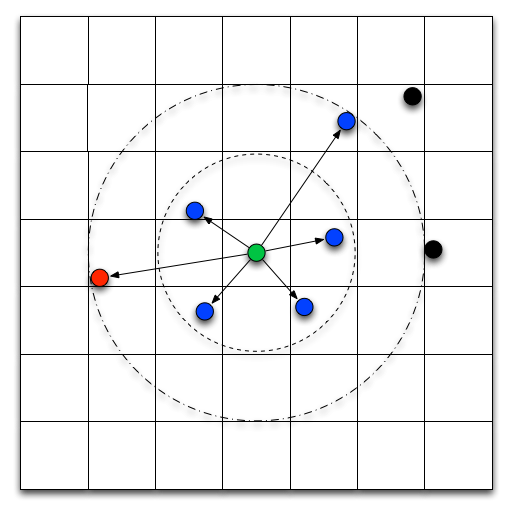
\includegraphics[width=6.5cm]{rbffd_methods_content/neighbors/ball_query_vs_kNN.png}
\caption{A stencil center in green finds neighboring stencil nodes in blue. Two ball queries are shown as dashed and dash-dot circles to demonstrate the added difficulty of finding the right query radius to obtain the $k$-nearest neighbors.}
\label{fig:nearest_neighbor_example}
\end{figure}


A na\"{i}ve approach to neighbor queries would be a brute-force search that checks distances from all nodes to every other node. Obviously the cost of such a method is high: $O(N^2)$. Multi-dimensional data structures can limit the scope of searching and reduce the cost of queries as low as $O(N)$. %TODO: correct lower bound? 


For the most part, investigations in RBF communities that delve into efficient neighbor queries are limited to work on the Partition of Unity method for approximation (e.g., \cite{Wendland2002,WendlandBook}) and particle methods like the Fast Multipole Method (e.g., \cite{Ying2006, Gumerov2003}) or Smoothed Particle Hydrodynamics (e.g., \cite{Krog2010}); all methods which depend on ball queries. Examples of fast algorithms employed these fields include the fixed-grid method \cite{WendlandBook,Krog2010}, $k$-D Trees \cite{WendlandBook}, Range Trees \cite{Wendland2002,WendlandBook}, and also $2^d$-Trees (i.e., Quad- and Octrees) \cite{Gumerov2003, Ying2006}. Surprisingly, while these other communities continue the quest for fast neighbor queries, RBF collocation and RBF-FD communities have been slow on the uptake. For many years, the standard in the RBF communities has been to use $k$-D Trees (see e.g., \cite{Fasshauer2007, FlyerLehto11,FornbergLehto11}). 


This chapter presents a novel algorithm to generate stencils for RBF-FD. It is based loosely on the fixed grid method from \cite{Krog2010}. \cite{Samet2005} would classify the algorithm as a \emph{fixed grid ``bucket" method with one-dimensional spatial ordering}. However, due to the use of spatial hashing to order nodes in memory it is referred to here as the \emph{Hash Algorithm}. 

The Hash Algorithm loosens the requirements for $k$-nearest neighbors ($k$-NN) stencils to allow $k$-``approximately nearest" neighbors ($k$-ANN). It also reorders nodes according to space-filling curves. In what follows, the Hash Algorithm is compared to an efficient implementation of $k$-D Tree (\cite{TagliasacchiMFE}). Benchmarks demonstrate that with the proper choice of parameters the Hash Algorithm is up to 2x faster than $k$-D Tree, and it comes with a free bonus: up to 5x faster SpMV on quasi-random nodes due to reordered nodes during the stencil queries. 


\section{$k$-D Tree}

Given a set of nodes in $d$-dimensional space, a $k$-D Tree partitions the data 
kD Trees partition 


$k$-D Trees can be constructed in $O(N \log N)$ time with each query resulting in a $O(\log N)$ cost \cite{WendlandBook}.


 when Wendland mentioned $k$-D tree as an option for ball queries in compact RBF partition of unity approximations---ironically the author opted to test two other data structures instead. Wendland later returned in \cite{WendlandBook} to fully describe $k$-D Tree for . 


In addition to $k$-D Trees, the author of \cite{WendlandBook} recommends two other data-structures that would be appropriate for RBF methods: a fixed-grid method, and $bd$-trees. While justification for both alternatives is sound, to our knowledge neither have been applied to RBF-FD or other RBF PDE methods. Until now that is. This chapter introduces a novel neighbor query for the $k$-NN problem in RBF-FD based on the fixed-grid method. 

\cite{TagliasacchiMFE}. 
\cite{MatlabKDTreeSearcher}




\begin{itemize} 
\item Tree build algorithm
\item Query algorithm
\item Total complexity due to the fact that we only need to query stencils once, so the build and query times are joint. 
\end{itemize}
\cite{Fasshauer2007}

$k$-D Trees can be extended to use the concept of buckets \cite{Friedman1977}, although these have not been applied in the RBF community. 



\section{A Fixed-Grid Hashing Algorithm}

The implementation runs entirely on the CPU (\cite{Krog2010} runs on the GPU). 


 can be described as a \emph{fixed grid ``bucket" method with one-dimensional spatial ordering} as classified by \cite{Samet2005}. 

Our method can handle both ball queries and $k$-NN. For the former simply include all cells that lie within the radius. It will continue to be approximate due to rasterization effects, but the radius could be enforced by sorting nodes by distance and truncating by the actual radius. The $k$-NN is a more challenging problem, because it requires additional effort in the query step to expand the search range until the desired $n$ neighbors have been found. 

Our benchmarks and testing focus on the more challenging problem of $k$-NN


The algorithm introduced here is the same as the Fixed-Grid Method in \cite{WendlandBook}.     


\begin{figure}
\centering
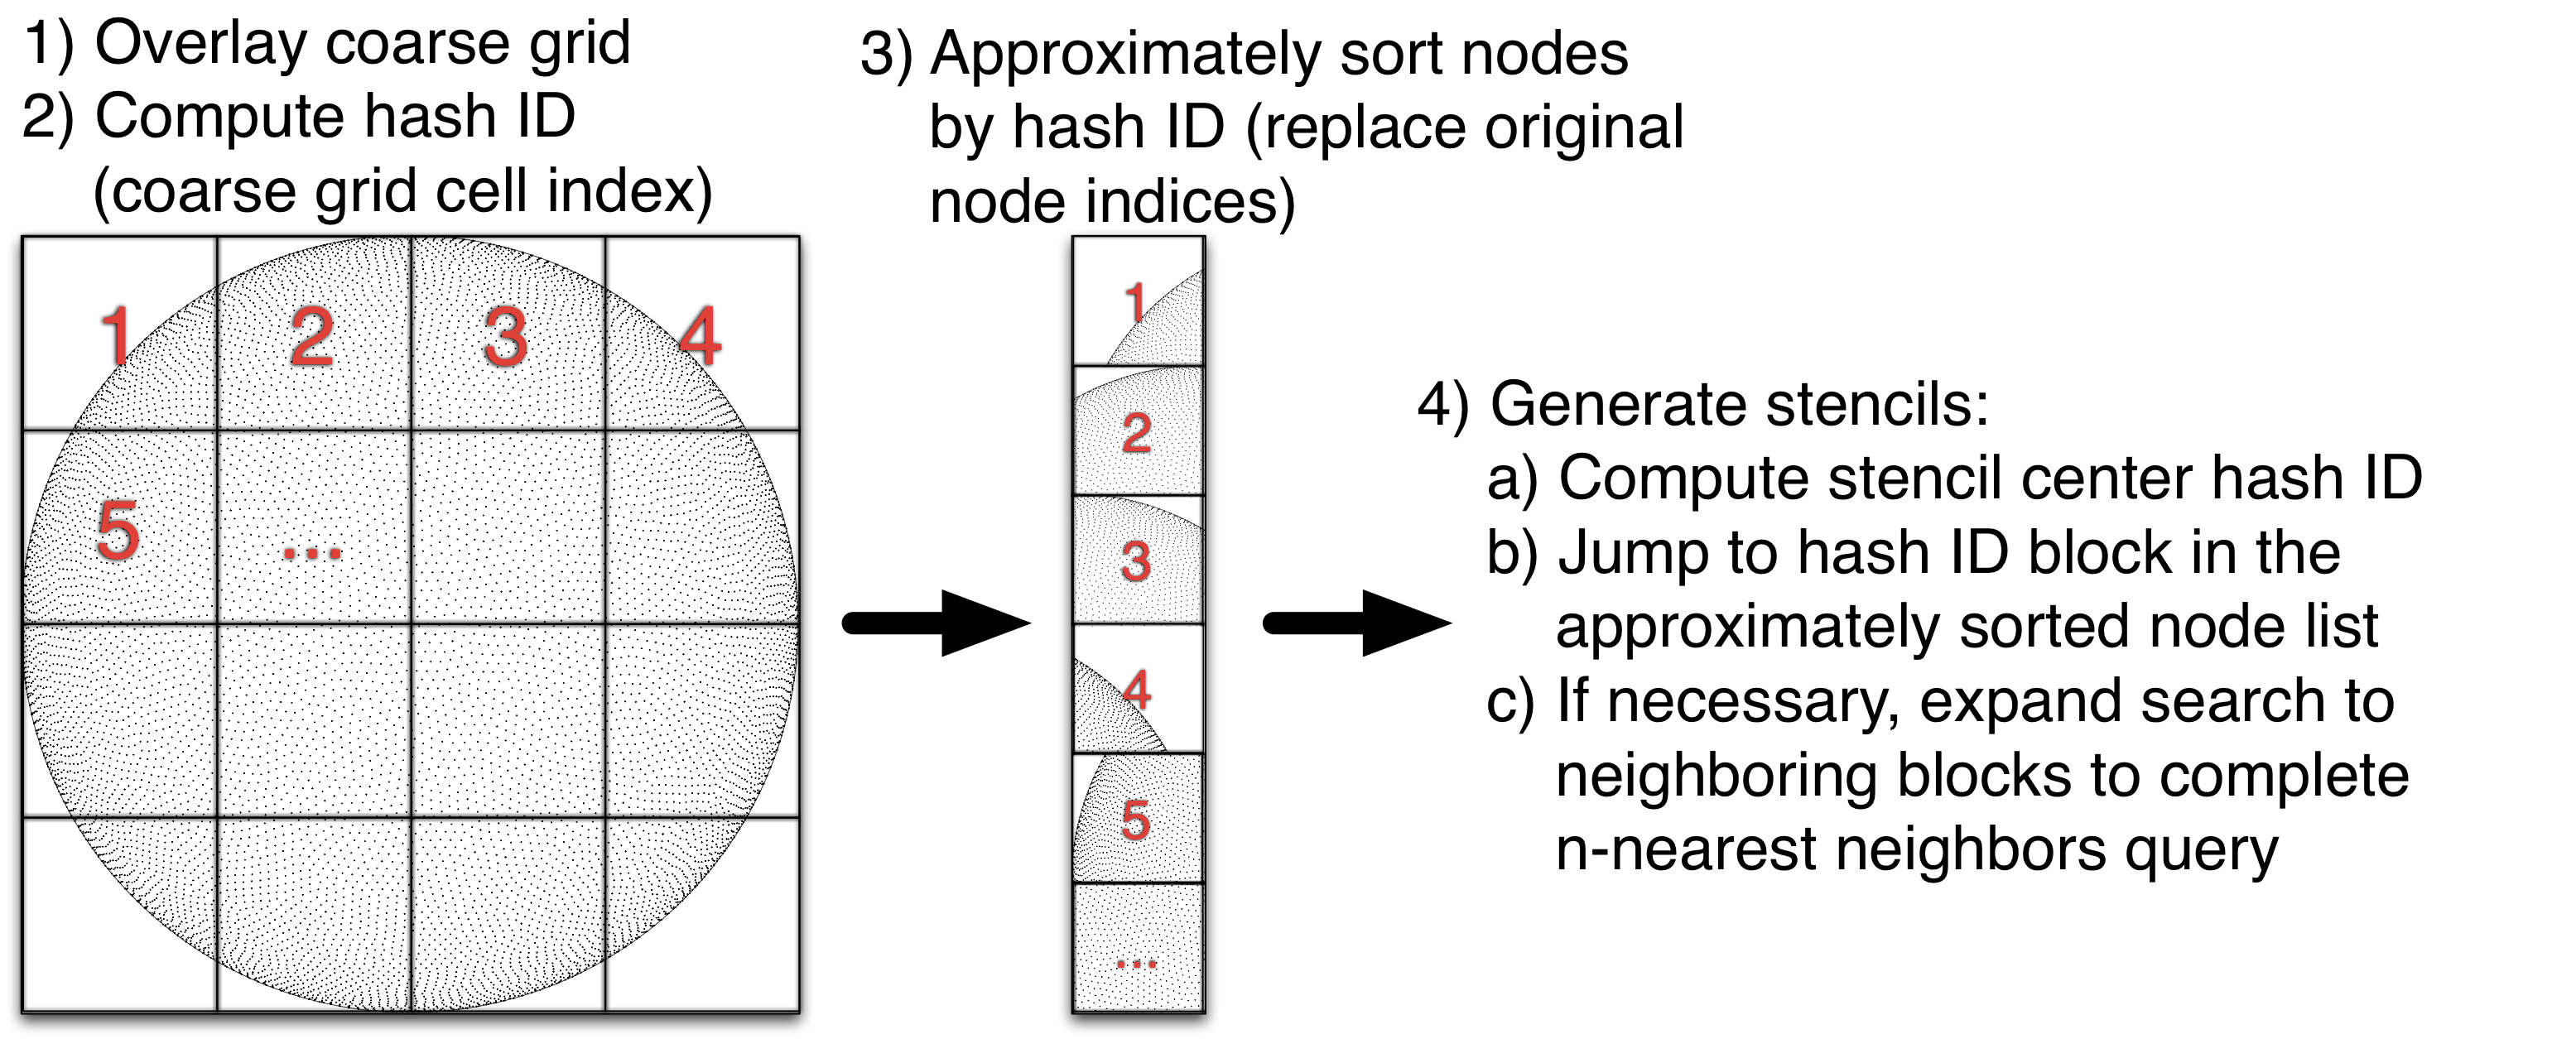
\includegraphics[width=1.0\textwidth]{../figures/chapter2/hashing_example/LSH_Concept.png}
\caption{High level overview of Locality Sensitive Hashing algorithm. First we overlay a coarse regular grid on the bounding box of the domain. The cells of the coarse grid cells are reordered in memory according to a space filling curve. Then we query neighbors by starting search with \authnote{Illustrate the query process} cell containing stencil center and append neighboring cells until stencil size $n$ nodes are found. We take $n$ closest neighbors (brute force search) if more than $n$ are appended to the list of candidates. }
\end{figure} 






Hashing, shown in Figure~\ref{fig:hashing_example} overlays a regular grid. This is equivalent to an axis aligned bounding box AABB, with refinement. In other words, we form a quad-tree in 2D, an octree in 3D. The neighbor query starts with the cell in which $x_c$ resides. Since we use an axis aligned bounding box, this cell index is easily calculated given the coordinate and number of subdivisions in each dimension. Once the cell index is resolved, the stencil is populated by taking the $n$ nearest neighbors from within the current cell. If the cell does not contain sufficient number of nodes to fill the stencil, the search for neighbors expands to include the cells immediately adjoining the center cell, taking only the nearest nodes in the provided cells. The search continues to expand outward in a rasterized circle/sphere until $n$ is satisifed. This search is considered approximate because it can happen that a true nearest neighbor would lie in a cell that is is not included in the rasterized circle, and other nodes are substituted from the far reaches of the discretized grid.

%TODO: cite lagrangian sph knn
The complexity of the method is still higher than the more efficient implementations used by Lagrangian methods, but as demonstrated in Figure~\ref{sten_methods_compare} the savings are significant. Generating stencils for RBF-FD is a preprocessing cost, so we do not dedicate an excessive amount of attention to this algorithm. However, a few ideas that would improve: hilbert ordering, choose AABB resolution based on $N$ not user parameters, faster sorting, GPU implementation




\subsection{$k$-NN vs $k$-ANN} 

Start at the center cell and add the 8 cells immediately surrounding it. Add to this the 16 cells in the second halo for a total of 25 cells. 

So while a $k$-NN stencil of size $n=8$ in Figure~\ref{fig:nearest_neighbor_example} would contain the black node in the right-most column of the grid. The $k$-ANN generated a stencil of size $n=8$ would opt for the black node to the top right because it is in the second halo and accepted as ``closer" because the stencil can be satisfied without querying the extra 24 cells on the outermost halo. 


One of the easiest ways to reduce complexity of 


Therefore, it is not essential that stencils contain only nearest neighbors. Instead, one can acquire the \emph{approximate nearest neighbors}. Figure~\ref{fig:ann_example} demonstrates a case where a does not contain all nearest neighbors. As illustrated in the Figure, the ANN stencil and true nearest neighbor stencil differ by one node. THis is not dire


The query is approximate because nodes such as the white node in Figure~\ref{fig:nearest_neighbor_example} could be included in the stencil before 


RBF-FD operates on general node distributions. Historically, stencils are uniform in size ($n$) and generated by selecting the $(n-1)$ true nearest neighbors to a node $x_c$. This is a $k$-NN query. 

Alternative queries are possible: ball query and approximate nearest neighbor. The approximate is of particular interest because nodes closest to the stencil will always be selected, whereas the nodes further away have minimal influence so swapping out cant hurt. The justification in altering the selection is for reduced complexity in neighbor queries.  


\begin{figure}
\centering
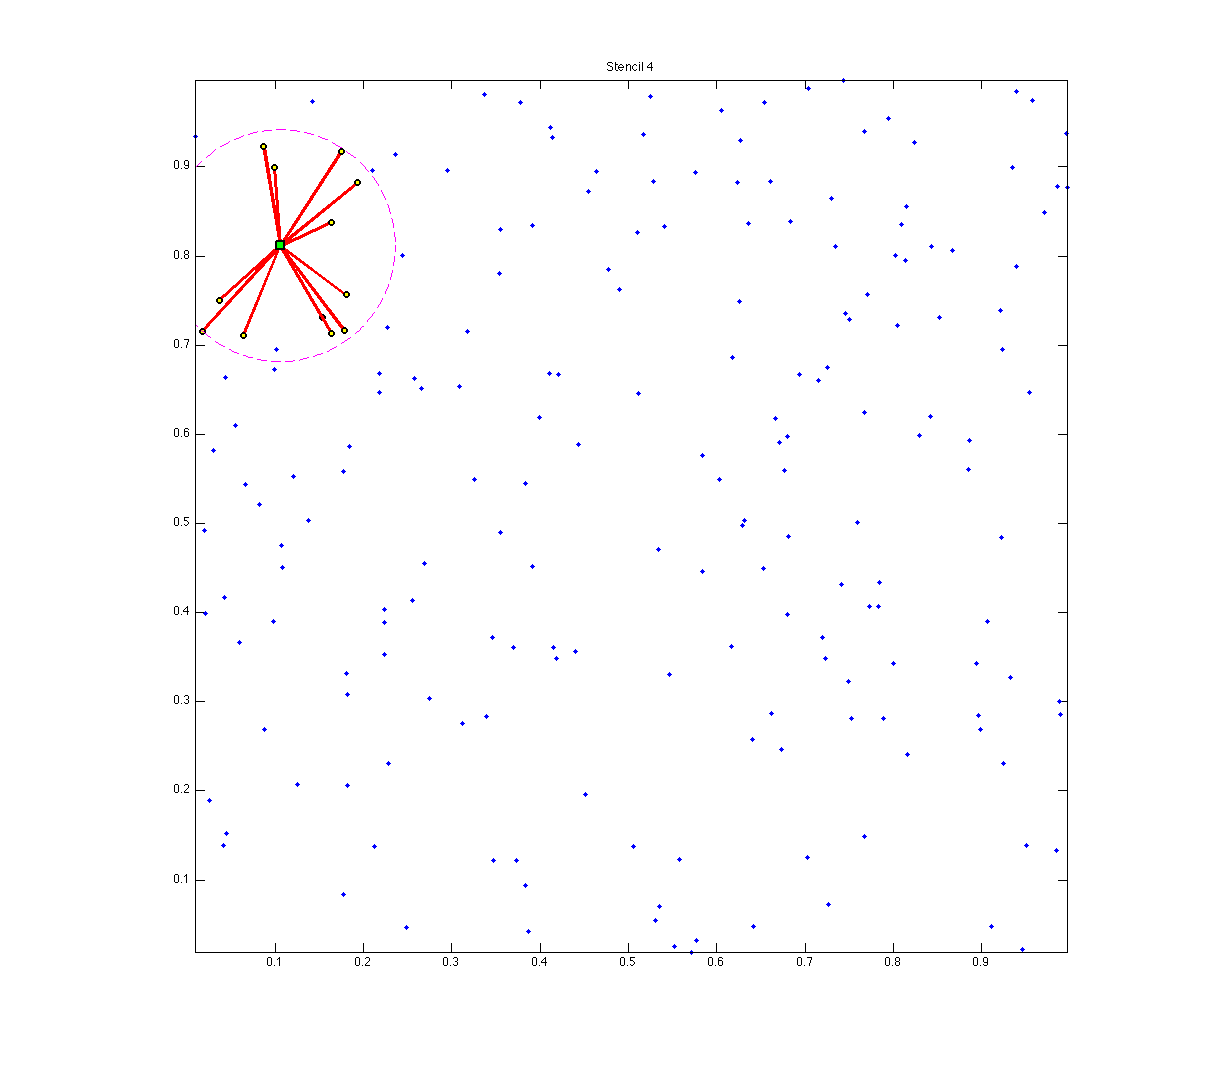
\includegraphics[width=8.5cm]{rbffd_methods_content/neighbors/neighbor_incorrect.png}
\caption{A stencil generated with $k$-ANN satisfies the required stencil size, but is not guaranteed to choose the true nearest neighbors.}
\label{fig:approximate_nearest_neighbors}
\end{figure}




\subsection{Integer Dilation and Node Reordering}


\begin{figure}
\centering
\begin{subfigure}{0.425\textwidth}
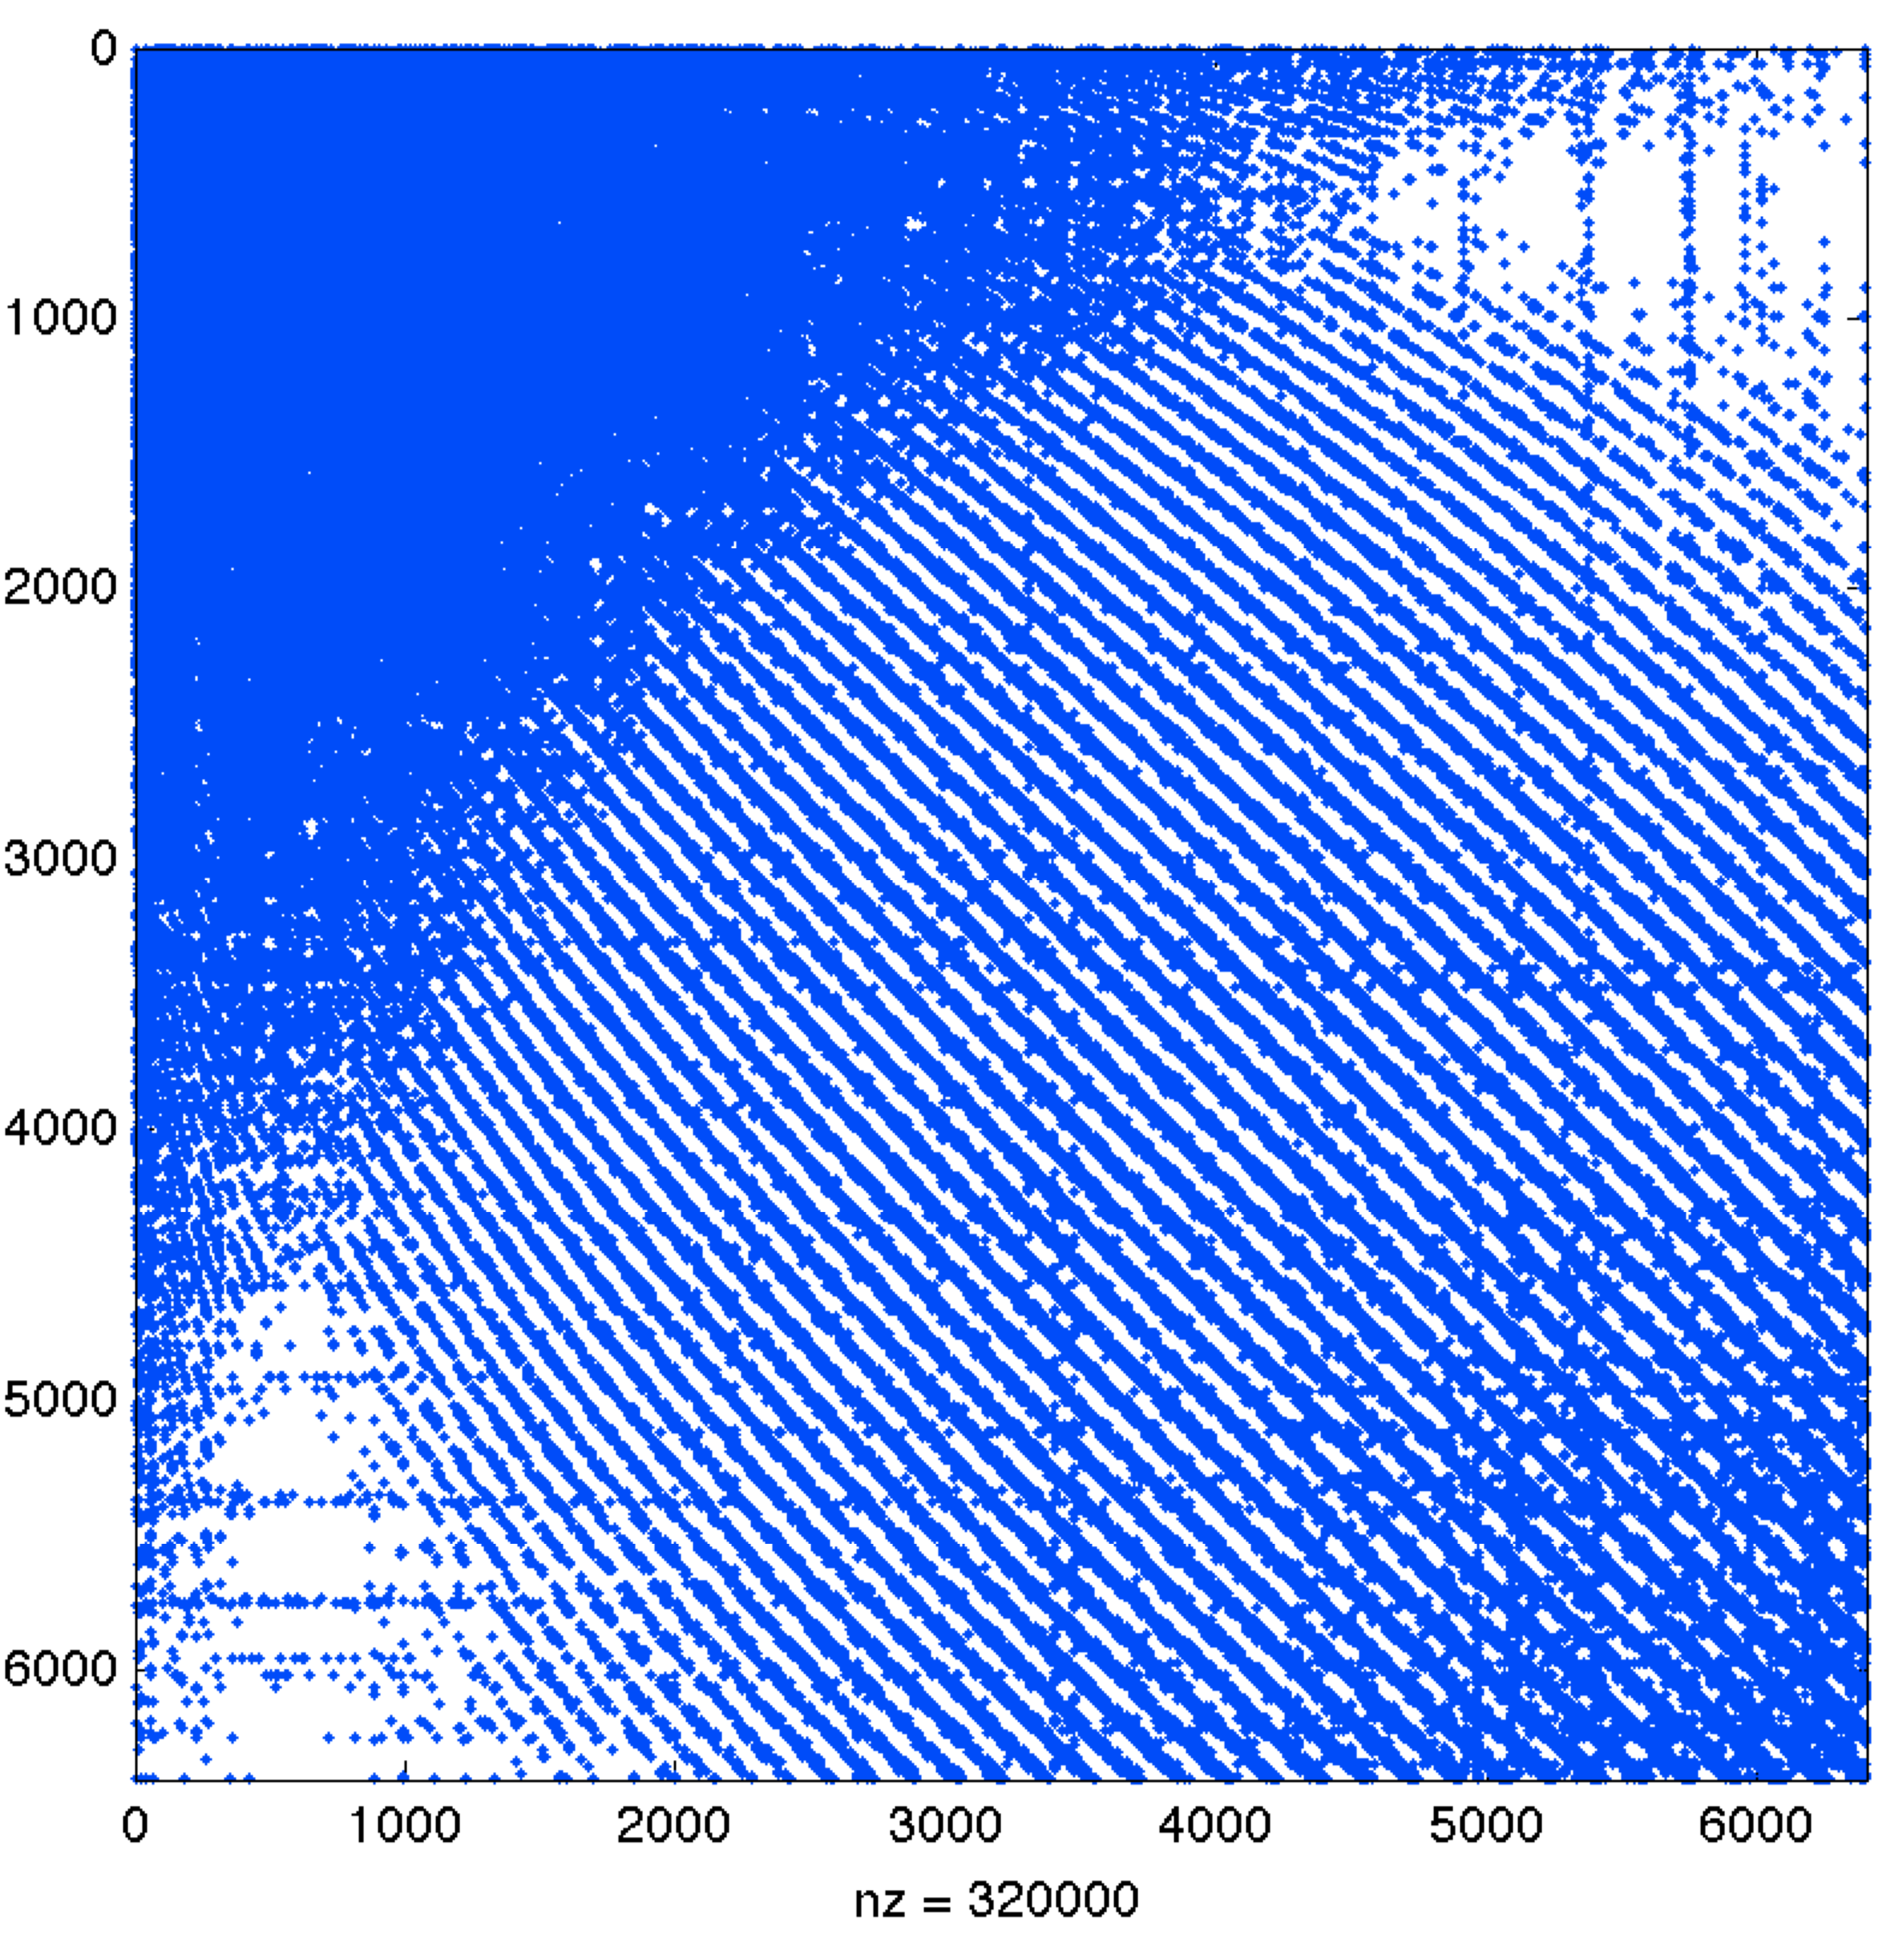
\includegraphics[width=1.0\textwidth]{../figures/chapter2/hashing_example/bruteforce_N6400_n50-eps-converted-to.png}
\caption{k-D Tree} 
\end{subfigure} 
\begin{subfigure}{0.425\textwidth}
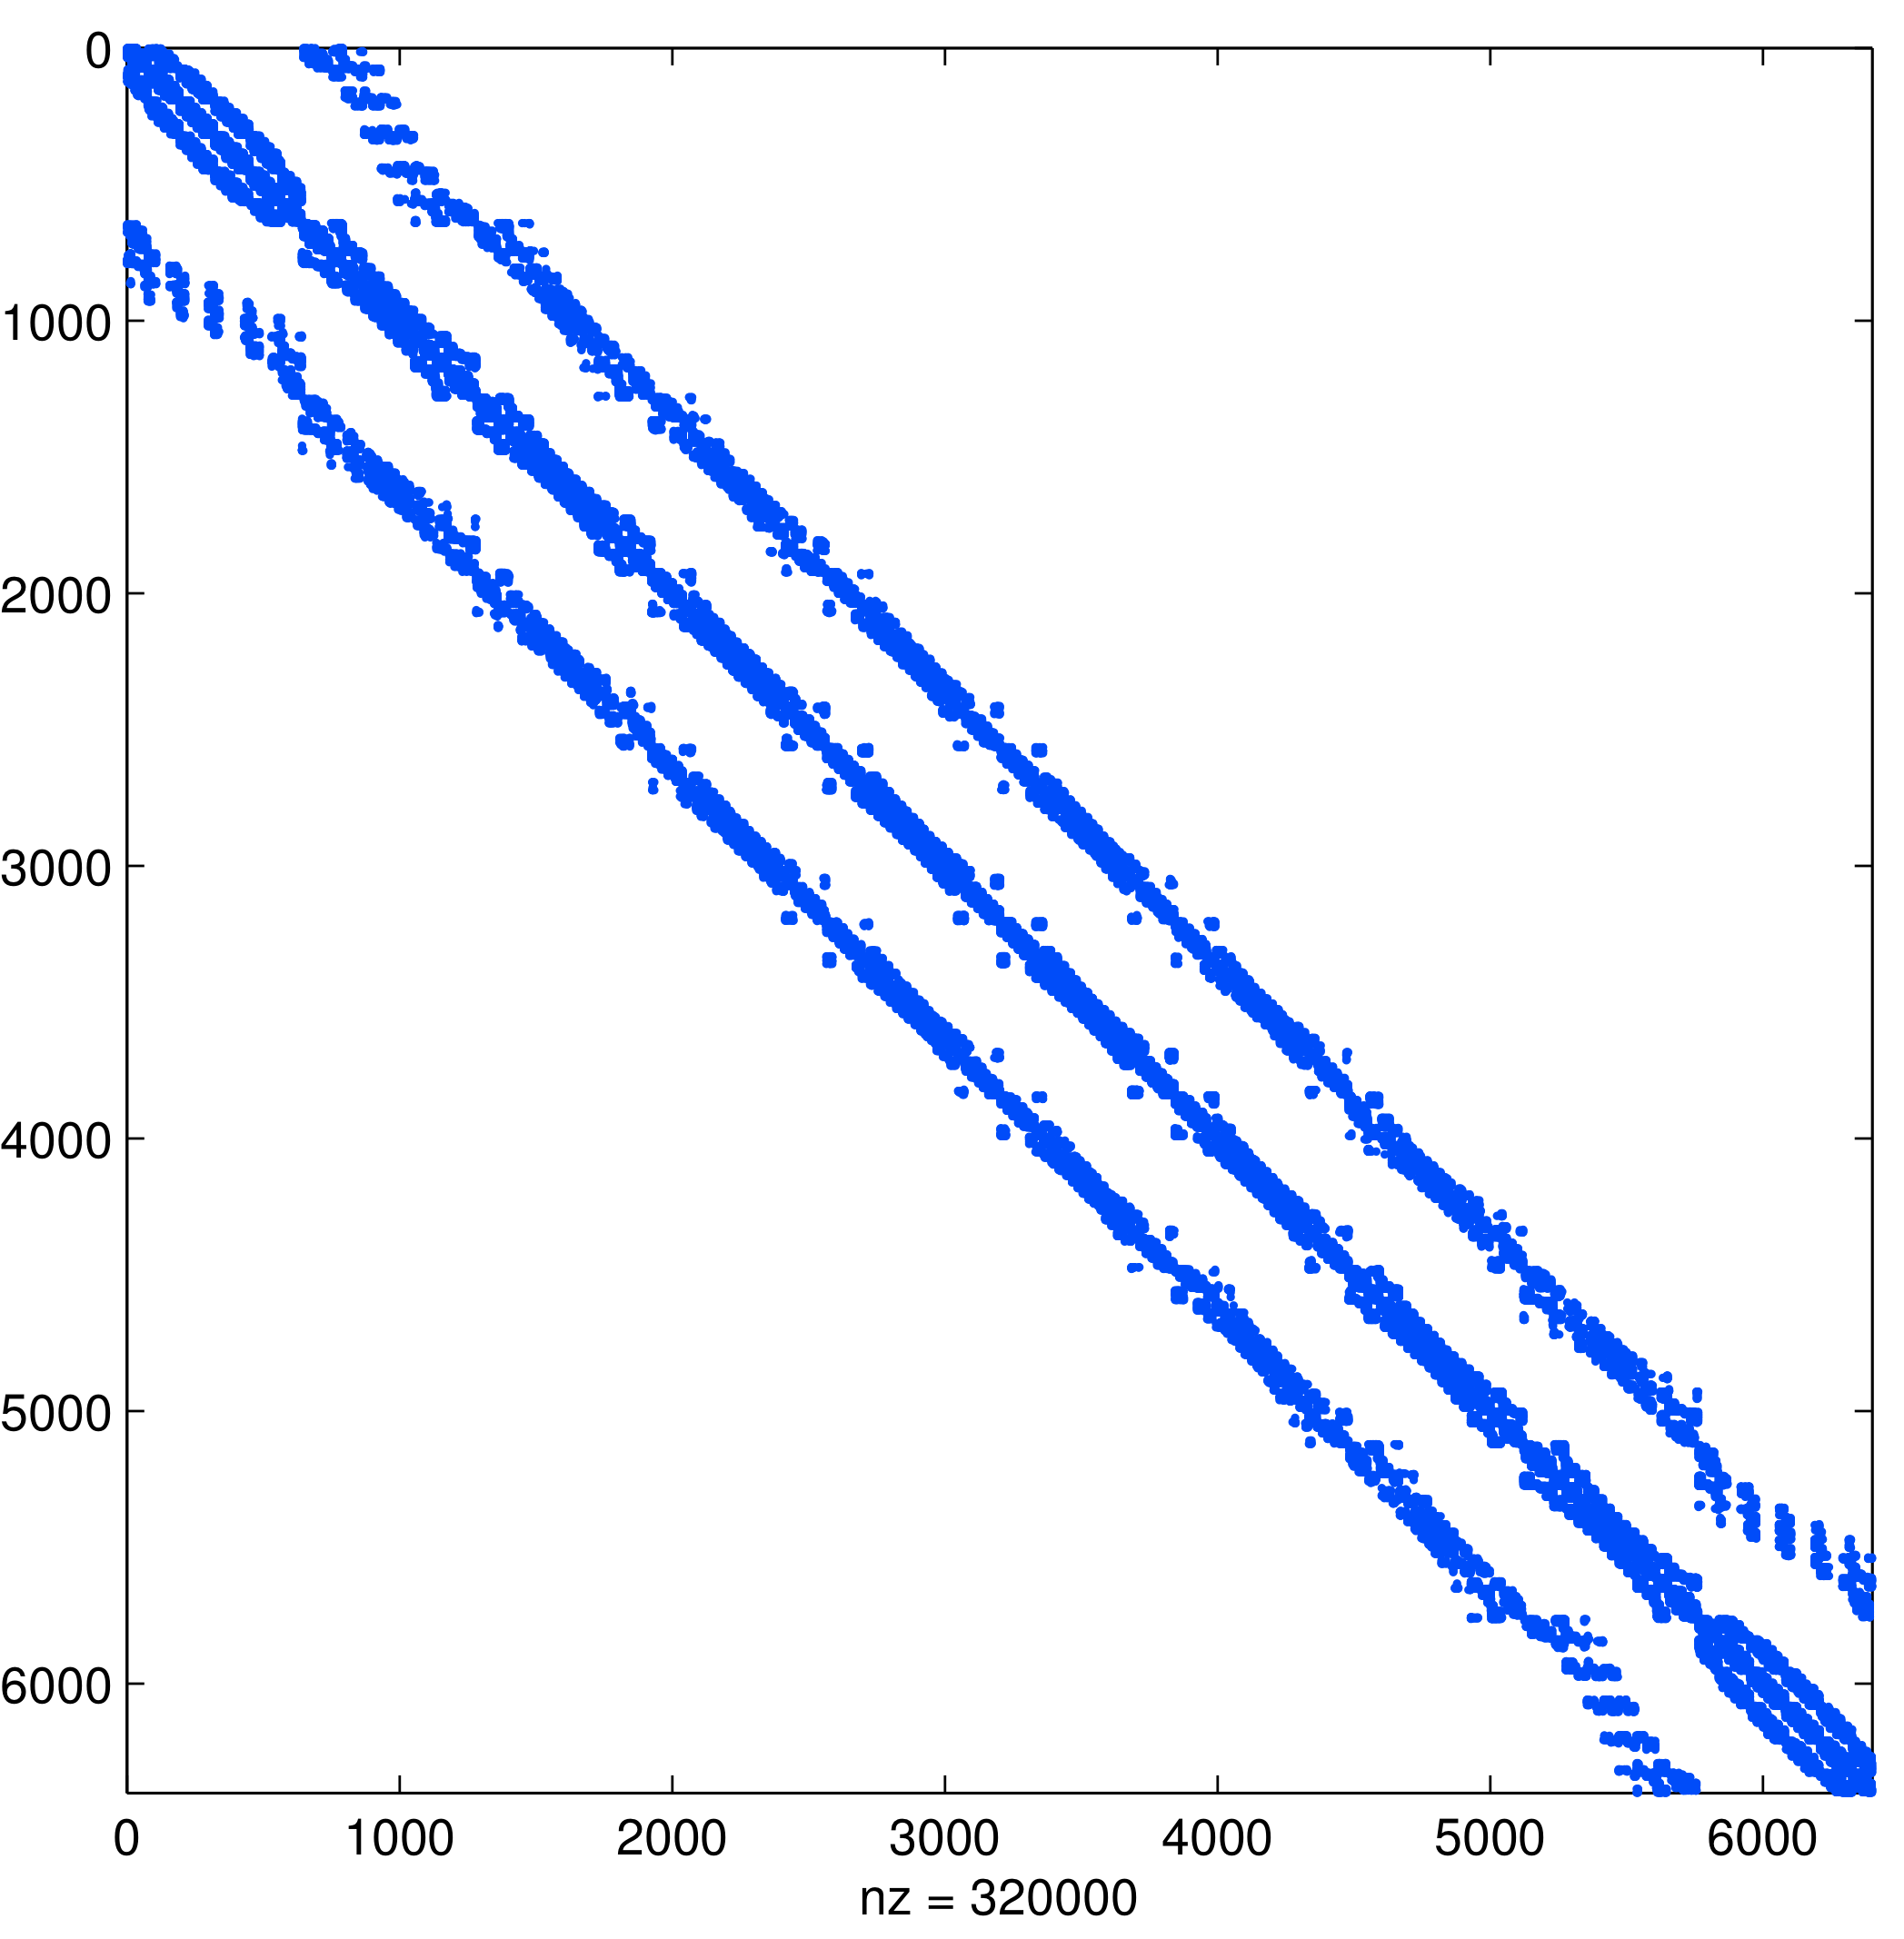
\includegraphics[width=1.0\textwidth]{../figures/chapter2/hashing_example/lsh_N6400_n50-eps-converted-to.png}
\caption{LSH}
\end{subfigure}
\caption{Example effects of node reordering within neighbor query algorithm for MD node set $N=6400$ with $n=50$. Matrix is $0.78\%$ full. k-D Tree maintains original ordering of the nodes and deceptively appears nearly dense. LSH algorithm reorders nodes according to raster ordering and reveals sparsity of the problem.  }
\end{figure} 

\cite{Samet2005} labels this type of algorithm as a \emph{fixed grid bucket algorithm} with the twist that it also has \emph{one dimensional ordering}
\begin{itemize} 
\item Algorithm to hash each node, push onto queue for each hash, sort by hash
\item Query by jumping to hash, building raster spheres
\item Need a good handle on the complexity. 
\item possibility to use space filling curves
\end{itemize}





\section{Performance Comparison}


At the start of this dissertation, the most widely used $k$-D Tree implementation in the RBF community was \cite{TagliasacchiMFE}. As a MEX-compiled 



\section{Conclusion}
\begin{itemize}
\item Performance improvement
\item SpMV impact
\item impact from space filling curves
\end{itemize}





Many algorithms exist to query the $k$-nearest neighbors (equivalently all nodes in the minimum/smallest enclosing circle). Some algorithms overlay a grid similar to Locality Sensitive Hashing and query such as... \cite{HarPeledMazumdar2003}.

Throughout the RBF community, one commonly finds $k$D-Trees in use for nearest neighbor queries. The data structure is recommended for its $O(N)$ complexity in querying nearby neighbors. 



For the purpose of generating RBF-FD stencils the $k$D-Tree is built and all queries are made once. There is no reuse of the tree so the build and query times are combined into one. 

TODO:
\begin{itemize}
\item Finish KDTree description
\item Hashing neighbor query algorithm description
\item Cite refs on multi-dim spatial data structures
\item Complexity of algorithms
\item impact from ordering on matrix sparsity. Bandwidth impact. Bandwidth impact on condition considered in future chapter. 
\item what is best overlay resolution? based on time to generate. choose resolution as n/2, n/9? etc? 
\item perform neighbor queries on raster order because its easiest to jump cells. then each cell can be reordered according to z,x,u, etc. for better memory locality. Matlab script to do this (can be ported to C)
\end{itemize}

With a grid present, stencils are generated by querying $n$ neighbors for each $N$ total nodes in the domain. While not required, one typically assumes a stencil of $n$ nodes must be the nearest neighbors to a stencil center. Afterall, as the distance between stencil nodes and the stencil center decreases, the accuracy of derivatives increases. 

Brute force searching for neighbors---computing the distance between every pair of nodes and then selecting the $n$ nearest---is discouraged due to its $O(N^2)$ complexity. Common practice in the RBF community is to construct $k$D-Trees to decrease the cost of queries (e.g., \cite{Fasshauer2007, FlyerLehto11, FornbergLehto11}). 

\authnote{Incomplete here to end of section}


Leveraging $k$D-Trees involves two costs: a) the initial tree construction, and b) $k$-nearest neighbor queries. 

GPU version of Locality Sensitive Hashing could reduce complexity further \cite{Pan2011}

This can be done efficiently using neighbor query algorithms or spatial partitioning data-structures such as Locality Sensitive Hashing (LSH) and $k$D-Tree. Different query algorithms often have a profound impact on the DM structure and memory access patterns. We choose a Raster ($ijk$) ordering LSH algorithm \cite{Bollig2011} leading to the matrix structure in Figures~\ref{fig:oneThreadPerStencil} and \ref{fig:oneWarpPerStencil}. While querying neighbors for each stencil is an embarrassingly parallel operation, the node sets used here are stationary and require stencil generation only once. Efficiency and parallelism for this task has little impact on the overall run-time of tests, which is dominated by the time-stepping. We preprocess node sets and generate stencils serially, then load stencils and nodes from disk at run-time. In contrast to the RBF-FD view of a static grid, Lagrangian/particle based PDE algorithms promote efficient parallel variants of LSH in order to accelerate querying neighbors at each time-step \cite{Pan2011, Goswami2010}. 


At the onset of our work on RBF-FD, the most commonly used KDTree implmentation used by the RBF community was \cite{Tagliasacchi2008}. Recently, improvements were made to the KDTree algorithm to reduce the cost of building the KDTree to $O(N log^2 N)$. 

Figure~\ref{fig:stencil_query_old_and_new} compares the total time to generate $N$ stencils of size $n=50$ with three methods: \cite{Tagliasacchi2008}, our hash-based neighbor query, and the improved KDTree from \cite{Tagliasacchi2012}. 
Until the new release of KDTree, our algorithm was a major improvement to the performance of stencil generation. The hash-based approach achieved greater than 


%RBF methods are traditionally described as general and meshless in that they apply to unstructured clouds of points in arbitrary dimensions. However, although the term meshless implies a method capable of operating with no node connectivity, all numerical methods---meshless RBF methods included---connect nodes in the domain. For example, the ``meshless'' global RBF method connects every node in the domain to all other nodes. Compact support or local RBF methods like RBF-FD limit connections to nodes that lie within a predetermined radius.

%The connections between nodes form a directed adjacency graph with edges that dictate the paths along which data/phenomena can travel. For example, a plus shaped stencil of five points with a center node and four neighboring nodes allows values to propagate north, south, east and west; not northeast, southeast, etc.


%They are robust and function on scattered point clouds. RBF-FD in particular requires stencils to be generated from $n$ nearest neighbors to a stencil center. The cost of these neighbor queries can vary greatly depending on the choice of algorithm or data-structure used to make the query. 

For example, in general brute force is inefficient 
The author of \cite{Fasshauer2007} queries $n$ nearest neighbors for a compact-support RBF partition of unity example with a $k$-D tree. In \cite{FlyerLehto11,FornbergLehto11} a $k$-D Tree is leveraged for all neighbor queries for RBF-FD. 

Our work in \cite{BolligFlyerErlebacher2012} leveraged an alternative to $k$-D tree, based loosely on space-filling curve orderings common in Lagrangian schemes like Smoothed Particle Hydrodynamics (e.g., \cite{IanThesis}, \cite{Kelager}). %TODO: I have used Locality Sensitive Hashing \cite{Indyk} in the past. According to Samet \cite{Samet "Multidimensional and Metric..."}, LSH uses a set of random hashes to assign indices for each node. Our case uses space-filling curve, so we use . 

Rather than iterate through all $N$ nodes to find the true neighbors, or step through a k-D tree in something like $O(log N)$ that requires extra built-out, ANN allows us to use a set of nodes that satisfy


\subsubsection{KDTree}
Most of the RBF community leverages the $k$-D tree, due to its low computational complexity for querying neighbors and its wide availability as standalone software in the public domain (e.g., matlab central has a few implementations for download, and the MATLAB Statistics Toolbox includes an efficient k-D Tree). 

The complexity of assembling he tree is

The Matlab central $k$-D Tree is MEX compiled and efficient. We integrated the standalone C++ code into our library.  

While the $k$-D Tree functions well for queries, its downfall is a large cost in preprocessing to build the tree. For moving nodes, such as in Lagrangian schemes, this cost is prohibitively high. In an attempt to reduce the cost, lagrangian schemes introduced approximate nearest neighbor queries based on 


\subsubsection{Hashing}

\section{Neighbor Queries} 

As part of the preprocessing stage for RBF-FD, the scattered point cloud must
be analyzed to generate stencils. To generate a stencil, any collection of
nodes can be selected. However, by choosing nodes close to the stencil center
and well balanced around it, we stand to get the best possible approximations
to derivatives. 

Why? well, the approximations are based on differences. Similar to classic FD,
draw a secant connecting two nodes of a stencil. The slope of the secant
determines the gradient at either point or a point in between. In the limit as
the points are moved closer to the same spot, the approximation to the
derivative at that point becomes exact. 

So ideally every RBF-FD stencil will operate on nearest neighbors. One way to
generate nearest neighbors is brute force $O(N^{2})$; very inefficient. 

Alternatives exist including k-D Tree

\subsection{k-D Tree}
Build complexity, seek times. Internal ordering 

We use implementation provided by Andrea Tagliasacchi \cite{tagliasacchi} as a MEX compiled set of routines for Matlab. These same routines are then linked into C/C++. 

\subsection{Locality Sensitive Hashing}

\cite{Connor2009} provide a fast parallel 

\cite{Henke2012} is working on parallel generation. \cite{IanJohnsonThesis} has OpenCL neighbor queries

We started with a CPU implementation to test appropriateness. 




Approximate nearest neighbors will be nearly balanced. 
We observe that RBF-FD functions as well on stencils of true nearest neighbors as it does on approximate nearest neighbors.

To demonstrate the savings in choice of stencil generation method, we provide Figure~\ref{fig:sten_methods_compare}. 
 

The impact of our neighbor query also extends influence on the structure of the RBF-FD DMs.
has is to To quantify the sparsity of a Differentiation Matrix we consider the ratio of non-zeros ($N*n$) to total elements in the matrix ($N^2$). For example, a problem of size $N = 10,000$ with stencil size $n=31$ has a ratio of $0.0031$ and is $99.69\%$ empty. 

Querying neighbors requires searching at least the immediate cell one layer of neighbors. by including one extra layer we ensure that small stencils near the border of the immediate cell can pick up neighbors in adjacent cells.


%TODO: sparsity
%TODO: Node ordering
%TODO: show blocks for boundary conditions (annulus)

A prototype implementation of this method allowed for a variety of space filling curves to reorder the cells. The curves are created through integer dilation \cite{IntegerD} 


\begin{figure}
\centering
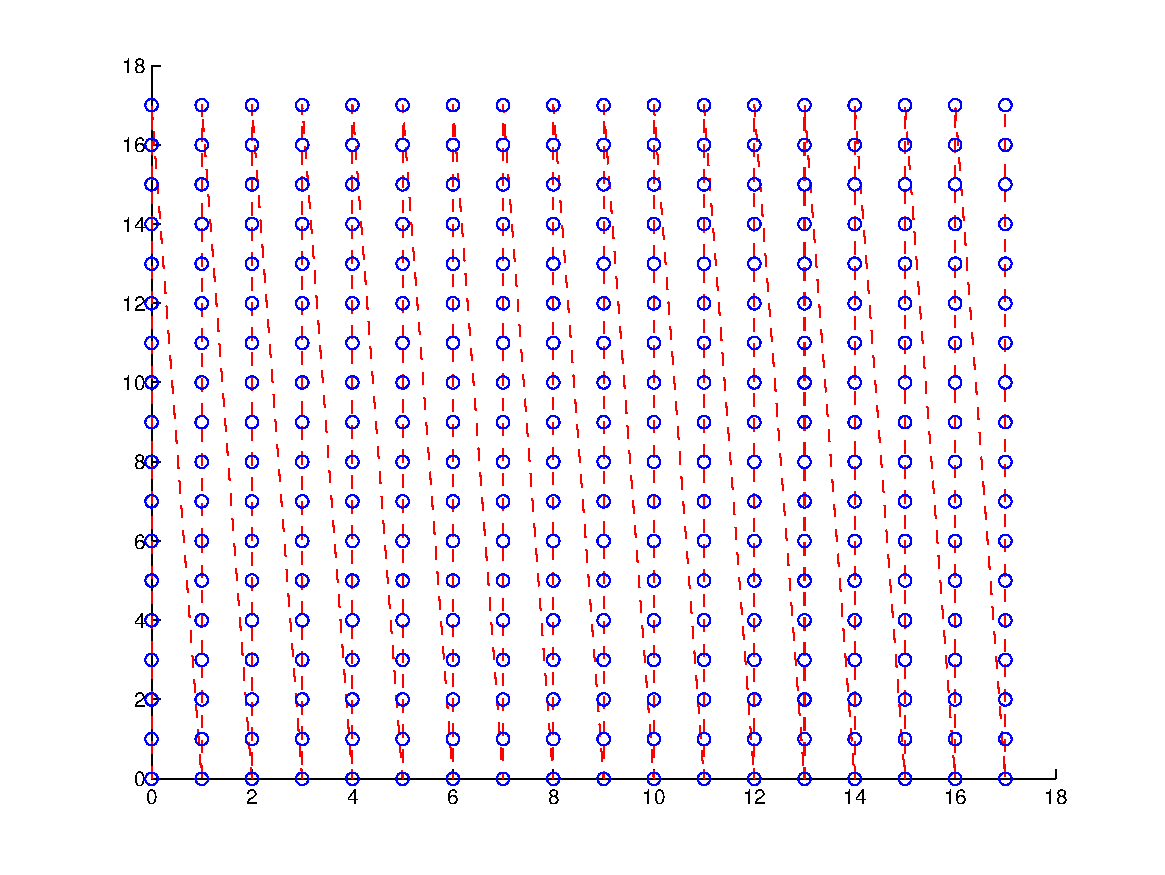
\includegraphics[width=0.45\textwidth]{rbffd_methods_content/hashing/originalorder_regulargrid-eps-converted-to.pdf}
\caption{In order: a) node ordering test cases; b) original ordering of regular grid (raster); c) coarse grid overlay for hash functions ($hnx = 6$); d) example stencil ($n=31$) spanning multiple Z's; e) spy of DM after orderings. \authnote{REGENERATE FIGURES WITH RANDOM/HALTON NODES}}
\label{fig:orderings}
\end{figure}

\begin{figure}
\centering
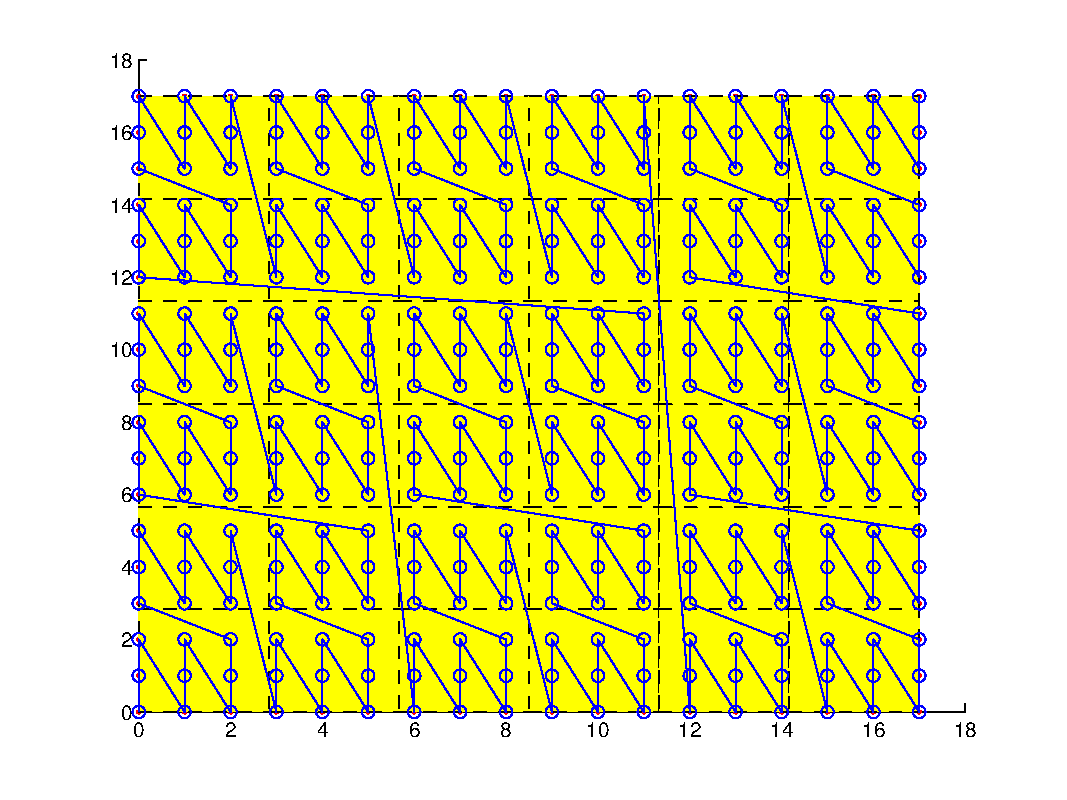
\includegraphics[width=0.45\textwidth]{rbffd_methods_content/hashing/overlay_regulargrid-eps-converted-to.pdf} 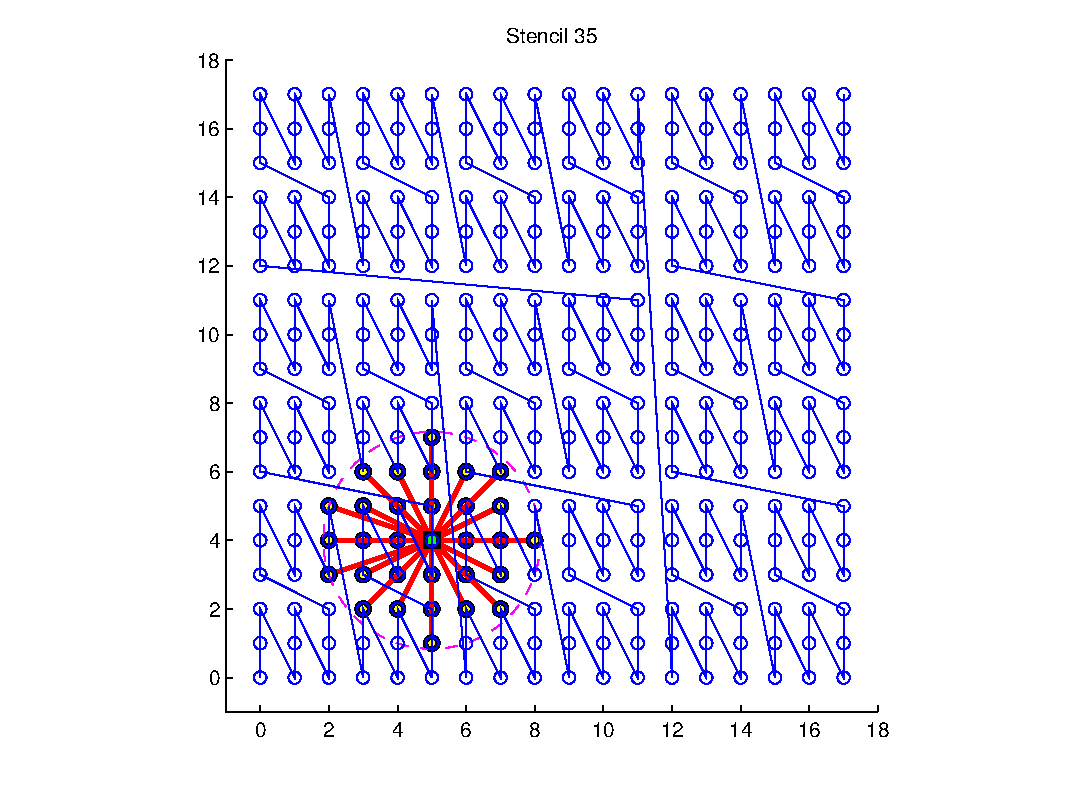
\includegraphics[width=0.45\textwidth]{rbffd_methods_content/hashing/stencil_regulargrid-eps-converted-to.pdf}
\caption{In order: a) node ordering test cases; b) original ordering of regular grid (raster); c) coarse grid overlay for hash functions ($hnx = 6$); d) example stencil ($n=31$) spanning multiple Z's; e) spy of DM after orderings. }
\label{fig:orderings}
\end{figure}

The KDTree implementation used in this work is from 

Original data showed our algorithm as wildly successful against a version  

The Cuthill McKee algorithms can be equated to a breadth-first search. The algorithm queues nodes in order of degree at each level of the search and traverses the lowest degree priority. The Reverse variant of Cuthill-McKee inverts the node order so that the lowest degree and top level node are at the end of the matrix rather than the beginning. Aside from ordering, the Reverse and Standard Cuthill McKee algorithms are identical processes. RCM is the more popular of the variants though, due to storage savings and reduced fill-in for some decompositions \cite{LiuSherman1976}.	. 
%TODO: get the compareKDTreeLSH.m output; this was for my C++ code and compared queries on 
%\begin{figure}
%\centering
%\includegraphics[width=0.65\textwidth]{rbffd_methods_content/hashing/
%\end{figure}



%TODO: \cite{Indyk "Algorithms for Nearest Neighbor Search"} for reference on quad vs kd vs lsh
%TODO: \cite{ChenChang "Neighbor-Finding Based on Space-Filling Curves"} 
%TODO: \cite{Stocco and Schrack "On Spatial Orders and Location Codes"}


Obviously, the ideal case for bandwidth is when all rows contain the $\frac{n}{2}$ nodes corresponding to solution value to either side of $u_j$. In 1-D this corresponds to every node containing the $\frac{n}{2}$ nodes to the left and right of $x_j$. In 2-D this is only possible if the nodes in the domain are properly indexed such that stencils contain the proper set of neighbors---a stringent requirement that will 


\begin{figure}
\centering
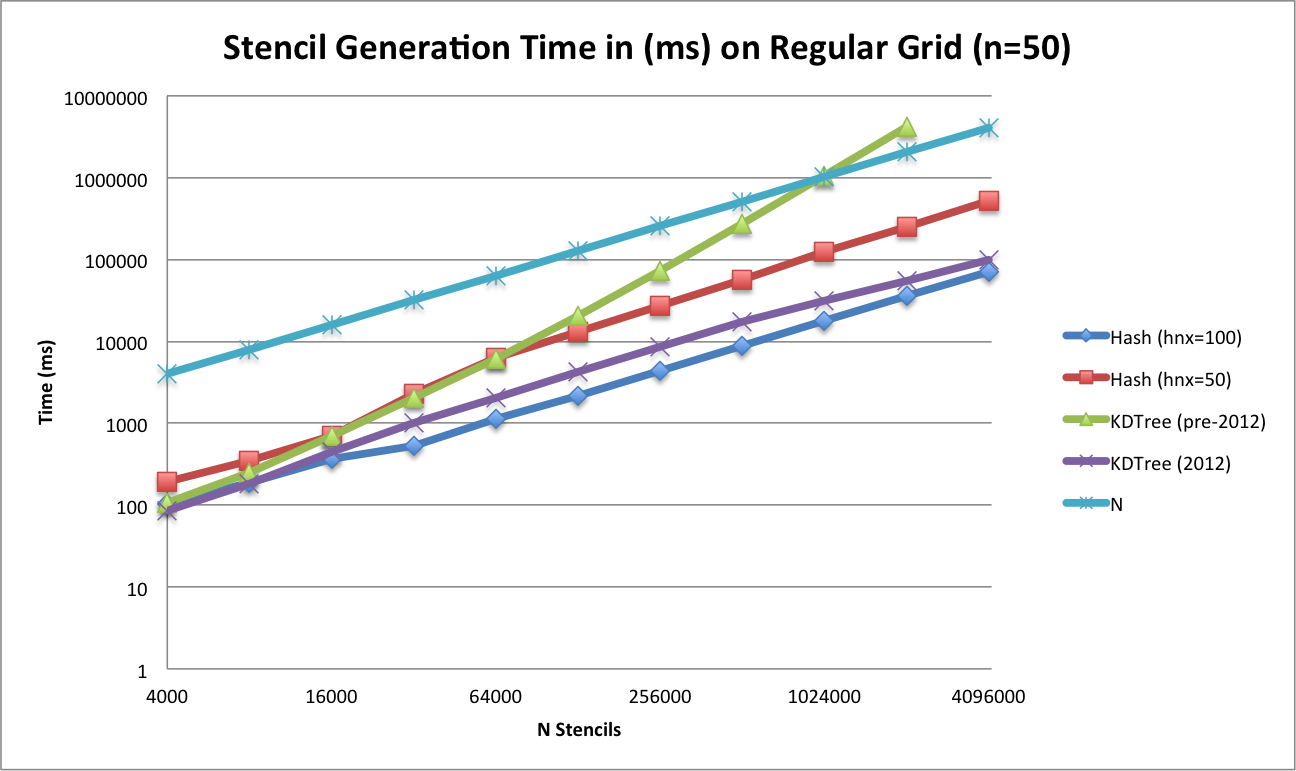
\includegraphics[width=9.5cm]{../figures/stencils/kdtree_old_reg_subsets_4m_stencil_gen_time.png}
%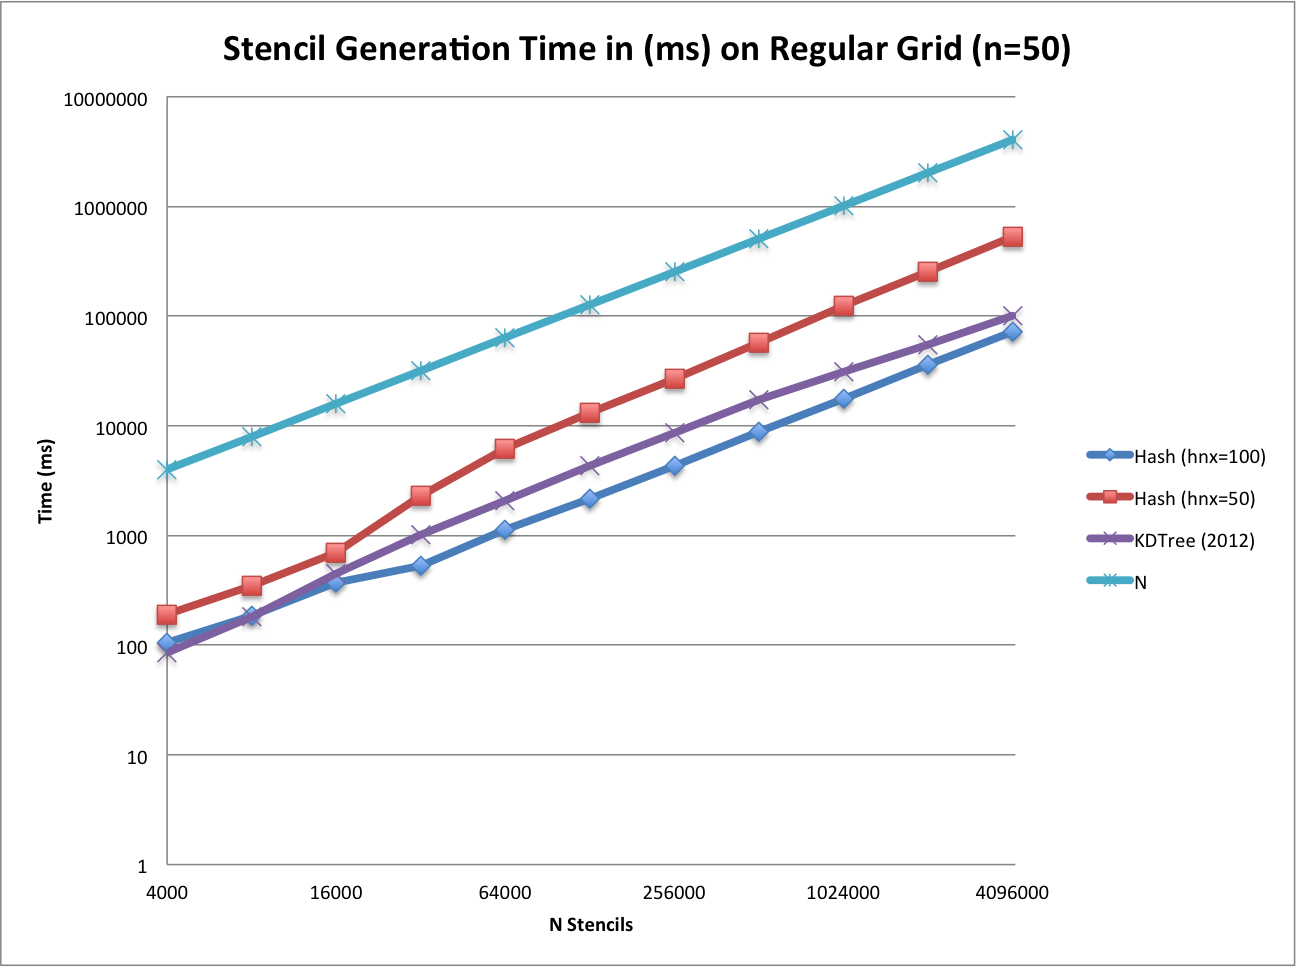
\includegraphics[width=9.5cm]{../figures/stencils/reg_subsets_4m_stencil_gen_time.png}
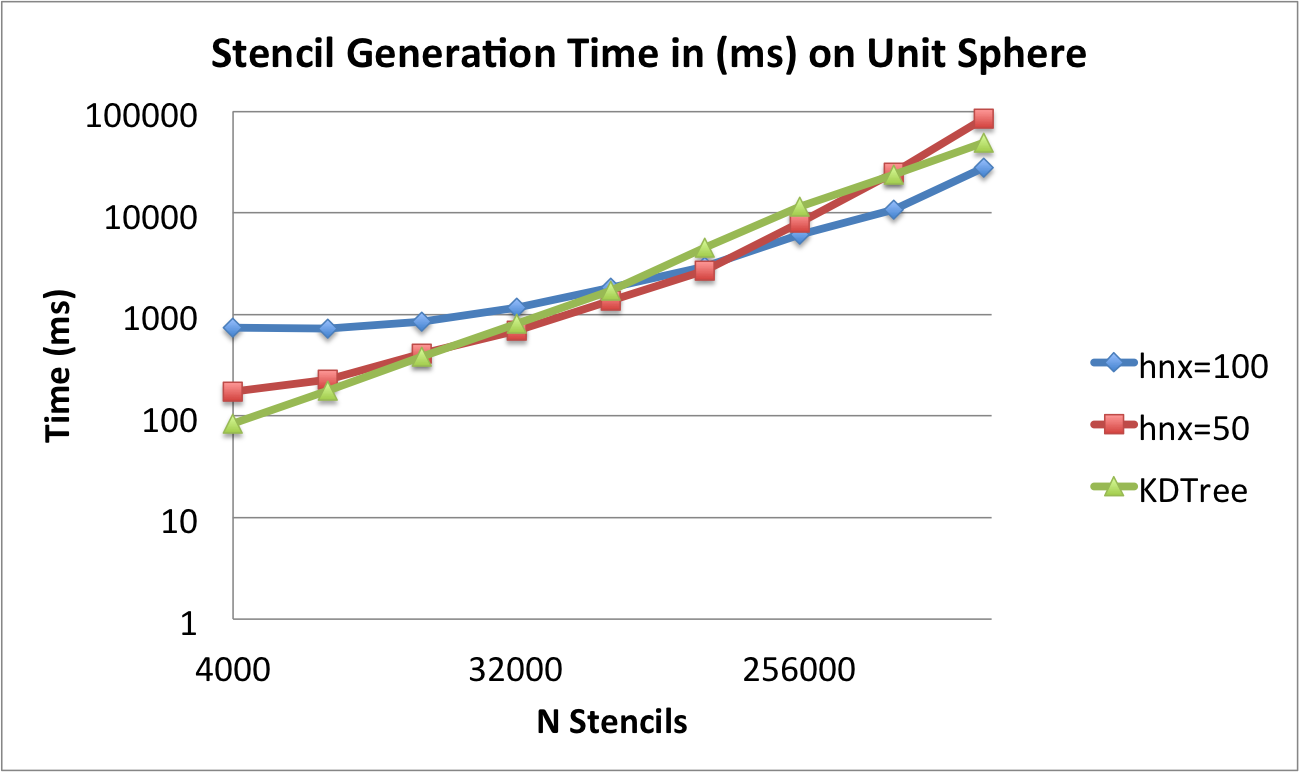
\includegraphics[width=9.5cm]{../figures/stencils/sphere_subsets_1m_stencil_gen_time.png}
\caption{Querying the $n=50$ nearest neighbors on a regular grid up to $N=160^3$ demonstrates the significant gains achieved by our spatially binned neighbor query. While KDTree queries grow as $O(N log N)$}
\label{fig:hash_results}
\end{figure}


The early implementation of $k$-D tree had an $O(n^2)$ growth in complexity. This algorithm was developed to alleviate that cost. It took a few hours to implement but has had some surprising impacts. Note that the complexity of $k$-D tree was reduced to $O(N \log^2 N)$ in 2012. On a regular grid (generated with raster/IJK ordering), the cost of $k$-D tree grows at the same rate as the hashing method. 

At $N=32000$ the cost of hashing drops below $k$-D Tree due to the decreasing number of empty hash cells. Likewise, at $N=1000000$ and beyond, the gap between hashing and $k$-D Tree begins to close as cells contain more than one 


Q: why does the curve drop for $hnx=100$? 
Q: the complexity of the algorithm? 
Q: the sphere I understand: its localizing the search to small patches on the sphere, and 





\begin{figure}
\centering
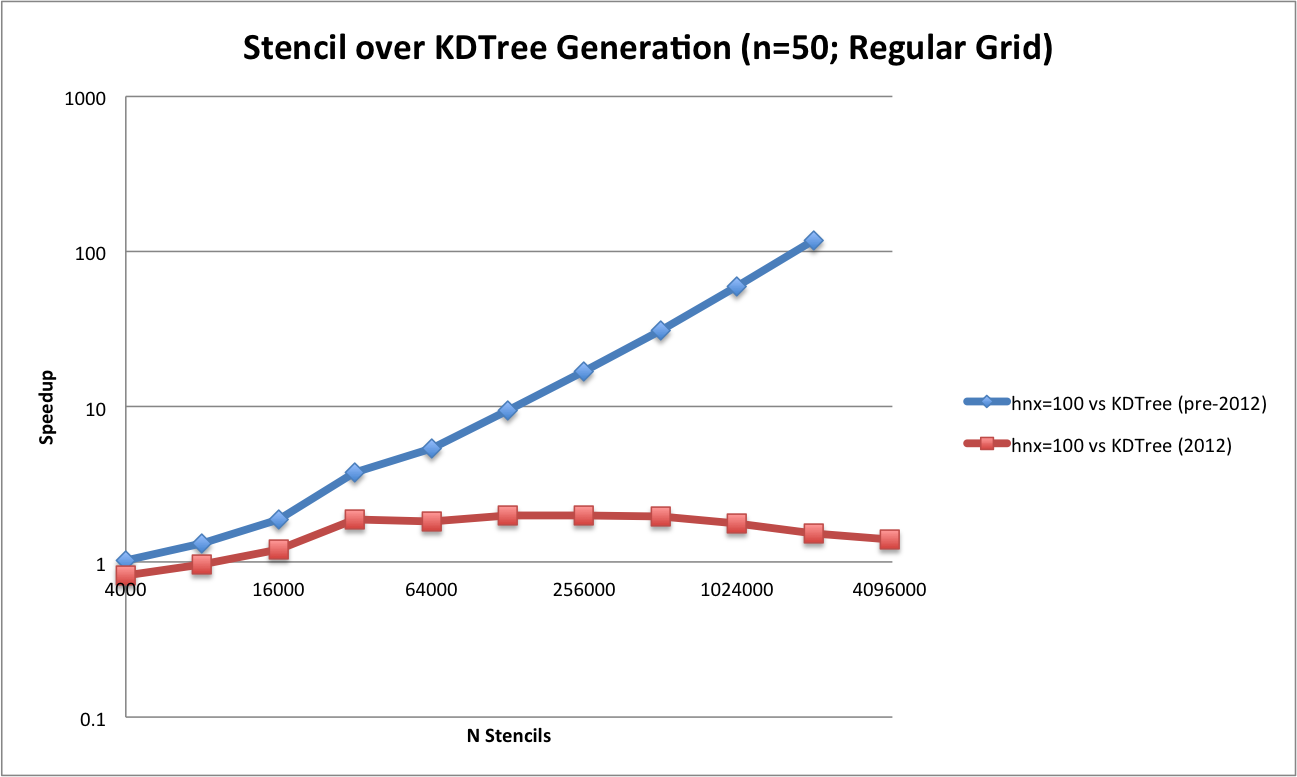
\includegraphics[width=9.5cm]{../figures/stencils/kdtree_old_reg_subsets_4m_stencil_gen_speedup.png}
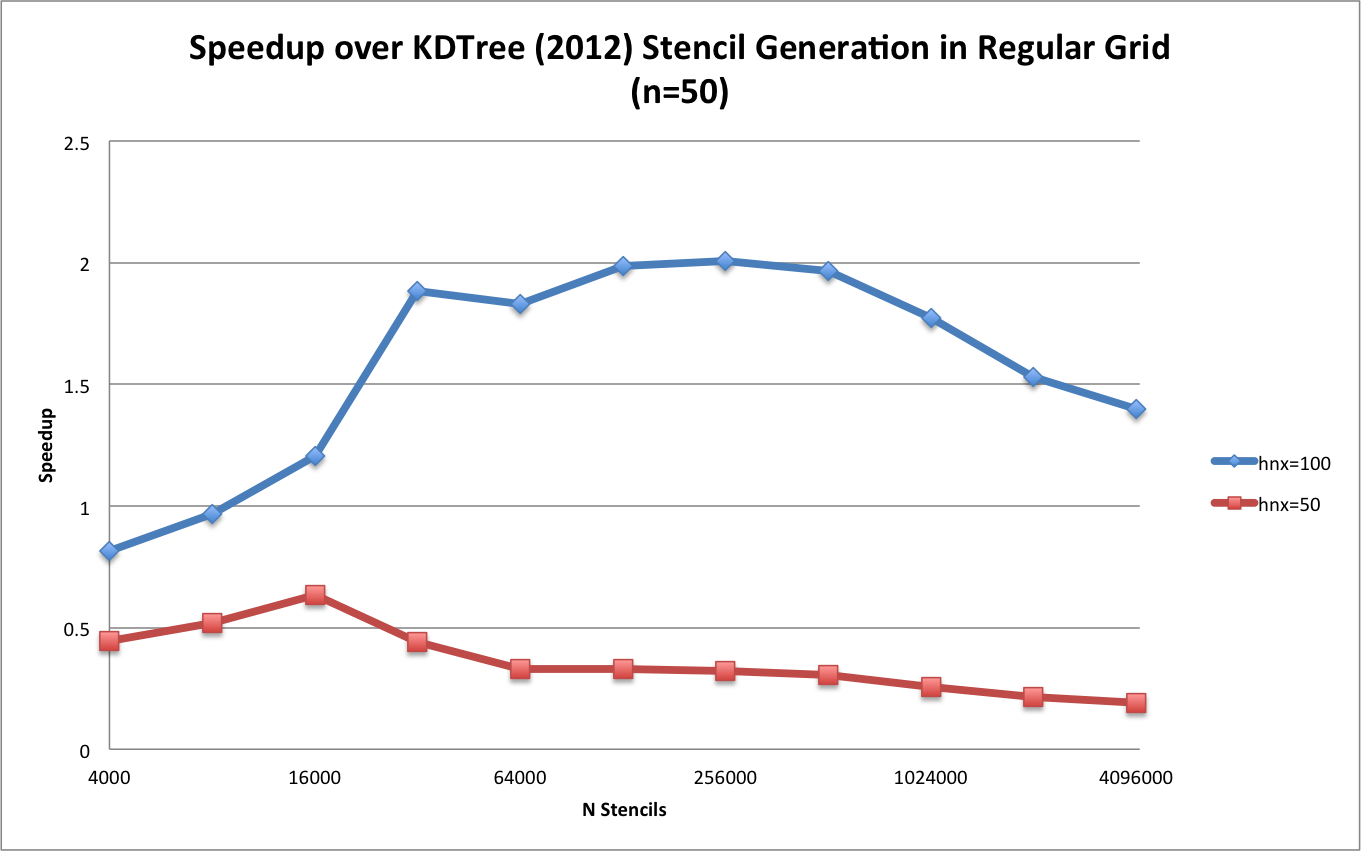
\includegraphics[width=9.5cm]{../figures/stencils/reg_subsets_4m_stencil_gen_speedup.png}
\caption{Querying the $n=50$ nearest neighbors on a regular grid up to $N=160^3$ demonstrates the significant gains achieved by our spatially binned neighbor query. While KDTree queries grow as $O(N log N)$}
\label{fig:hash_results}
\end{figure}
\begin{figure}
\centering
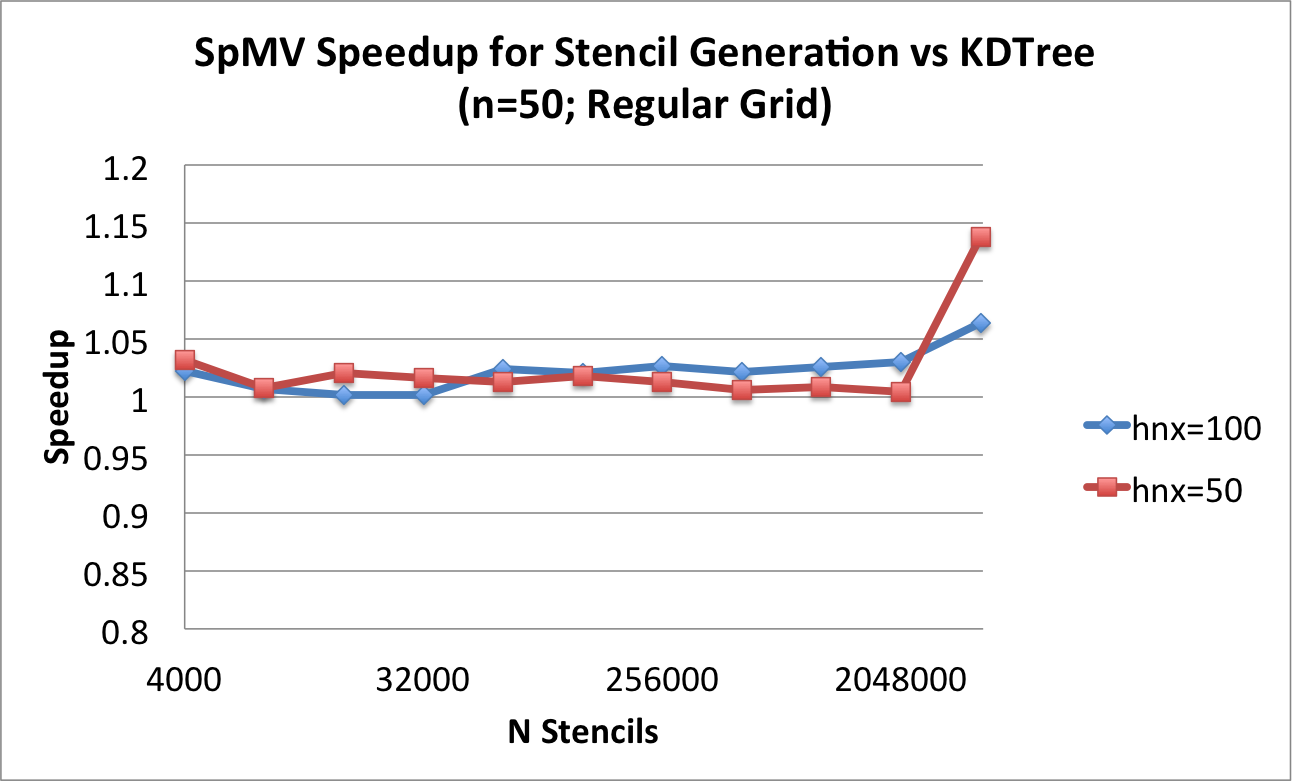
\includegraphics[width=9.5cm]{../figures/stencils/reg_subsets_4m_spmv_speedup.png}
\caption{Querying the $n=50$ nearest neighbors on a regular grid up to $N=160^3$ demonstrates the significant gains achieved by our spatially binned neighbor query. While KDTree queries grow as $O(N log N)$}
\label{fig:hash_results}
\end{figure}
\begin{figure}
\centering
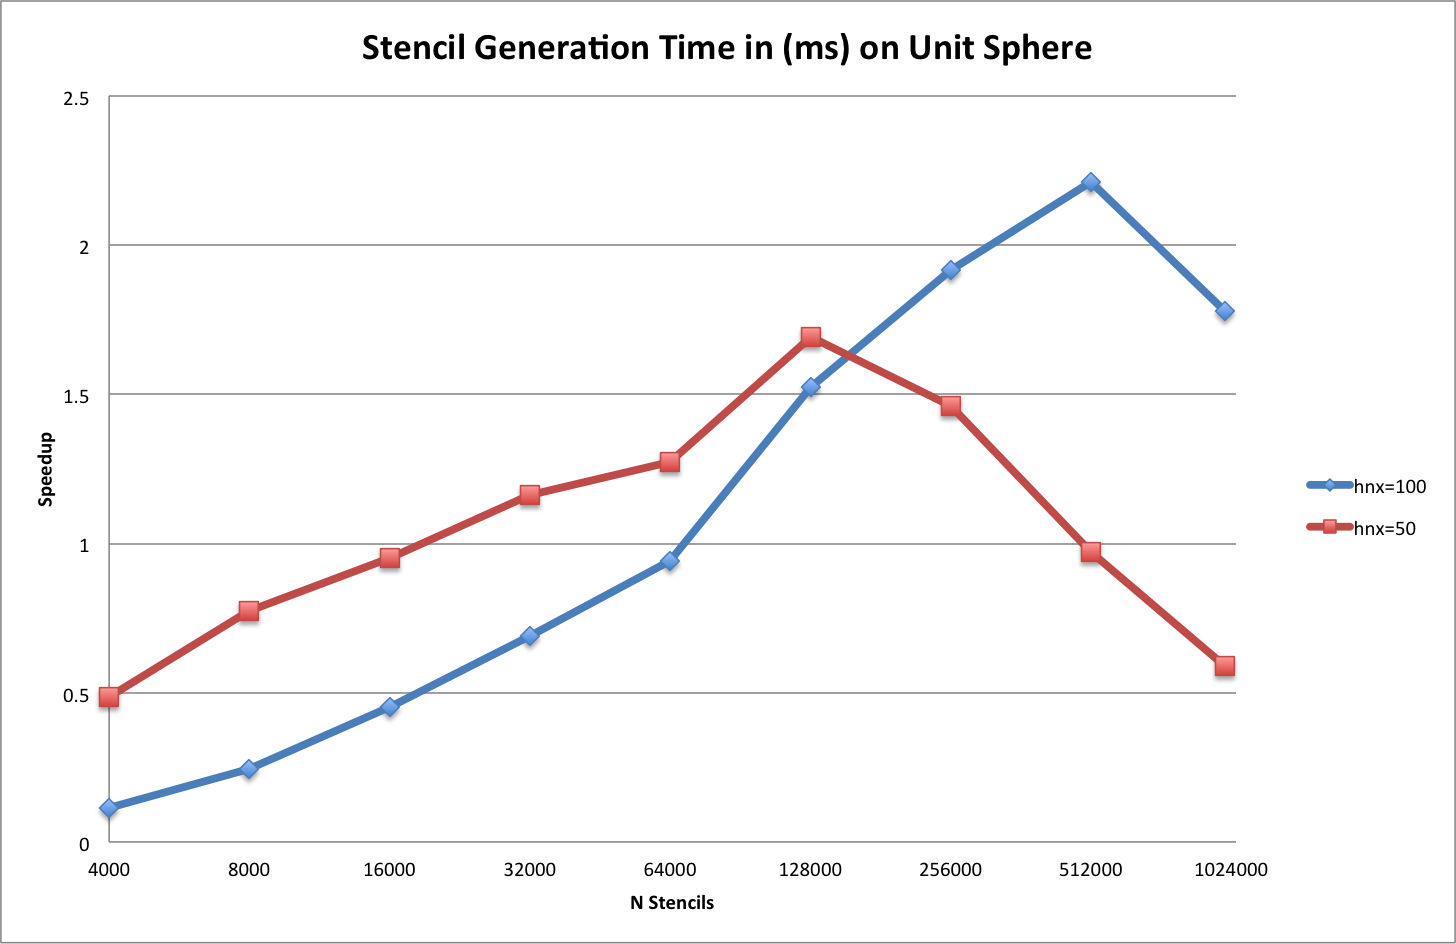
\includegraphics[width=7.5cm]{../figures/stencils/sphere_subsets_1m_stencil_gen_speedup.png}
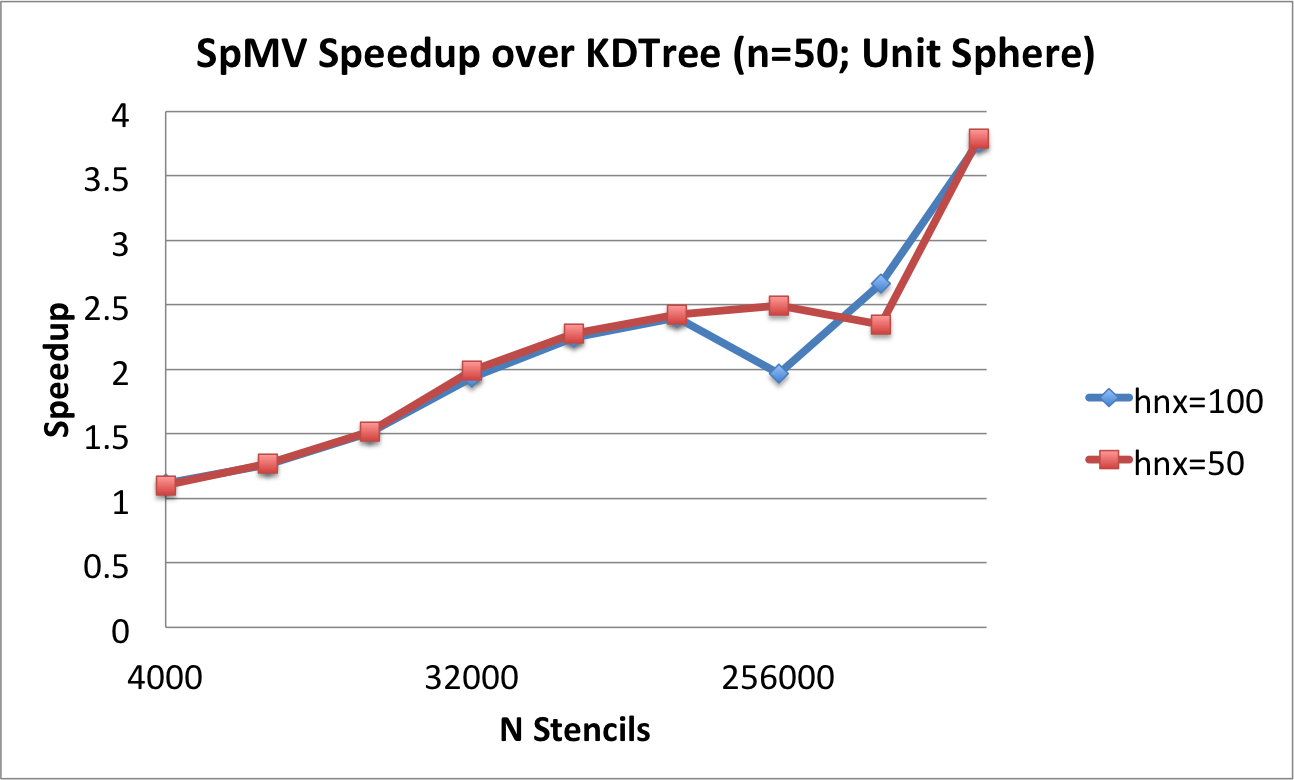
\includegraphics[width=7.5cm]{../figures/stencils/sphere_subsets_1m_spmv_speedup.png}
\caption{Generating stencils for increasing subsets of the $N=1e6$ CVT nodes mesh.}
\label{fig:hash_results}
\end{figure}
\begin{figure}
\centering
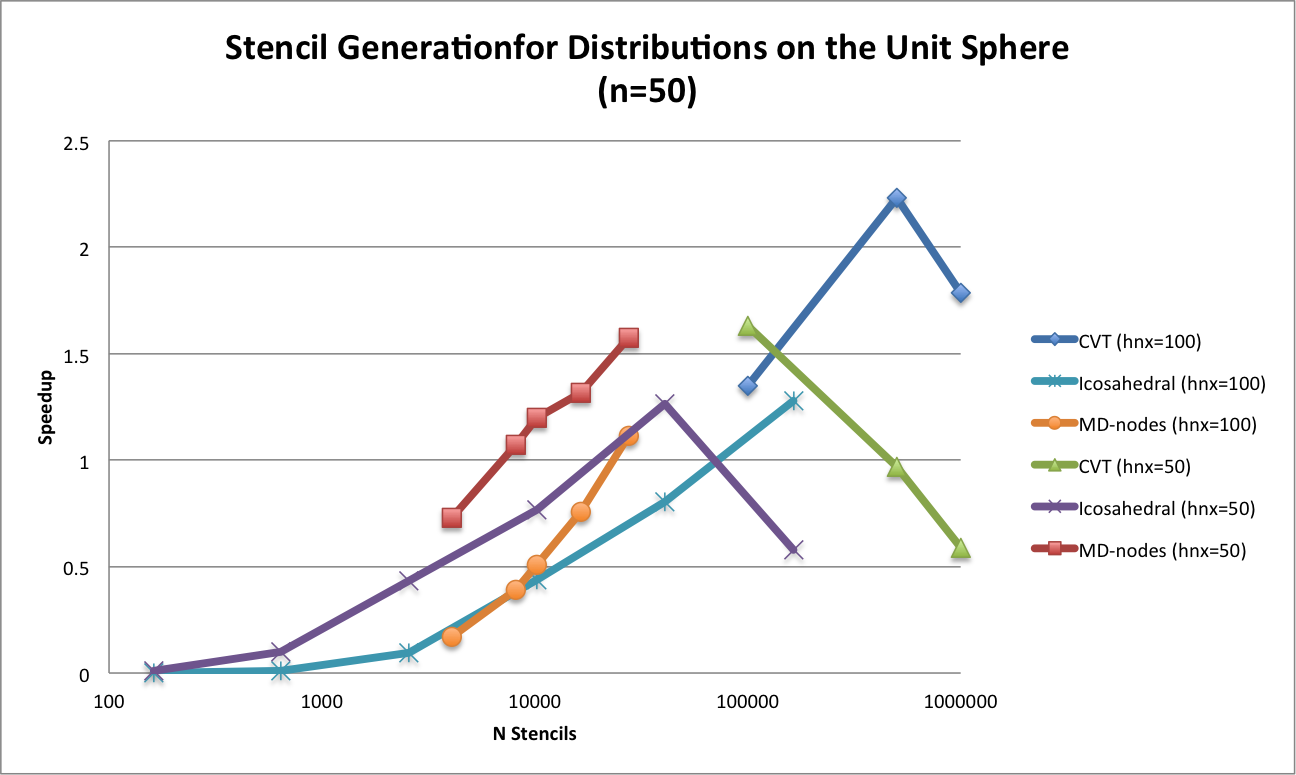
\includegraphics[width=10.5cm]{../figures/stencils/sphere_stencil_gen_speedup.png}
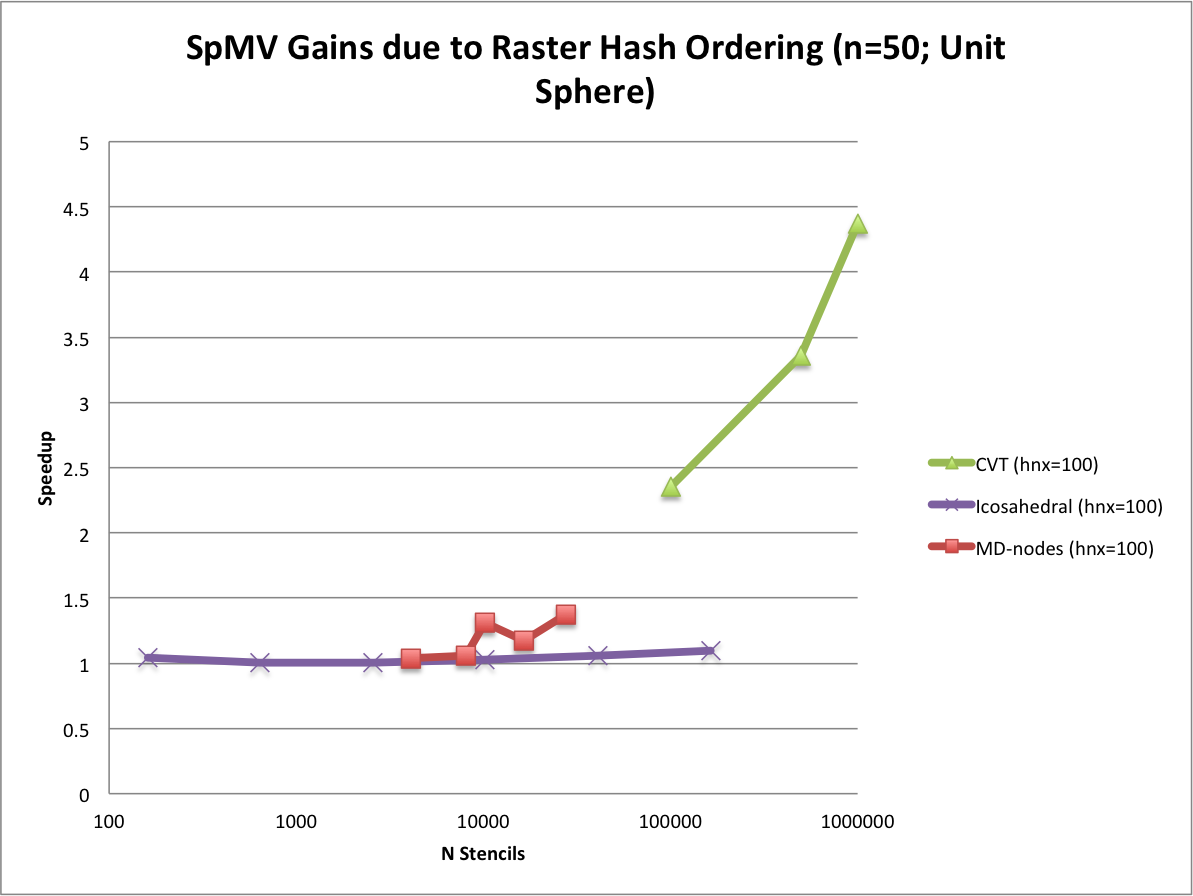
\includegraphics[width=10.5cm]{../figures/stencils/sphere_spmv_speedup.png} 
\caption{Based on the proper choice of overlay resolution, the hash stencil query can accelerate stencil generation, but the sophistication of the algorithm is low enough that negative impact is more likely. On the other hand, the impact on SpMV performance is always positive with the routine accelerated up to 4.9x faster.}
\label{fig:hash_results}
\end{figure}

\begin{figure}
\centering
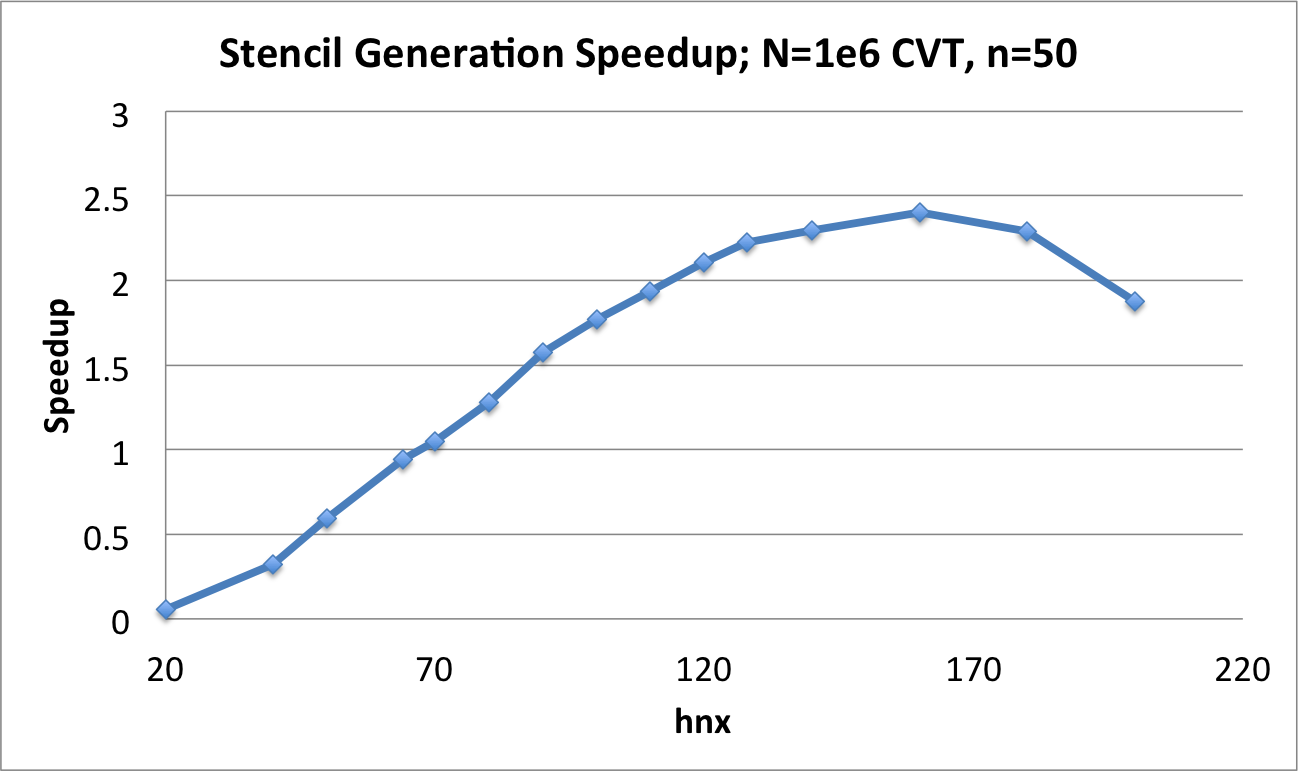
\includegraphics[width=7.5cm]{../figures/stencils/cvt1m_stencil_gen_speedup.png}
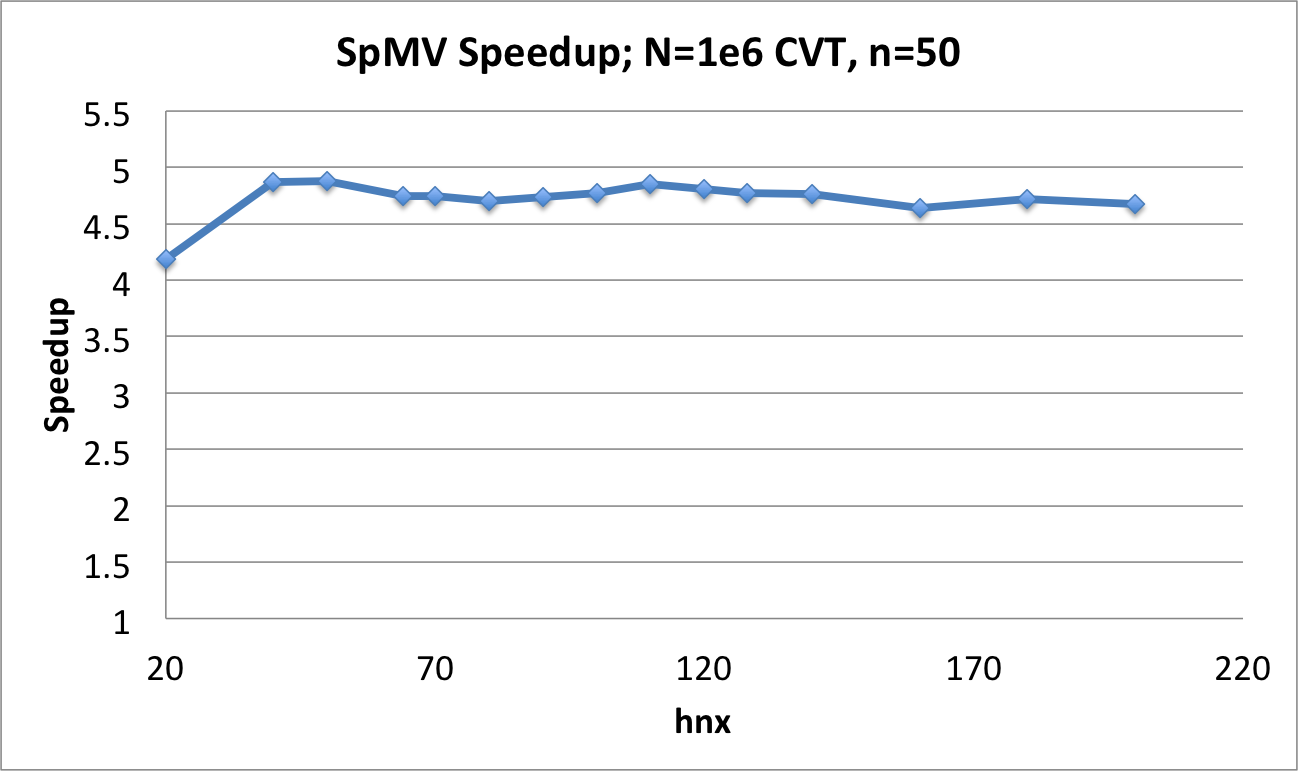
\includegraphics[width=7.5cm]{../figures/stencils/cvt1m_spmv_speedup.png} 
\caption{As the coarse grid resolution increases the hashing algorithm achieves both 2x faster than KDTree in stencil generation, with greater than 4x gain in SpMV performance (for free).}
\label{fig:hash_results}
\end{figure}

For every $N$ there is an optimal $hnx$. This is depicted for $N=500000$ CVT and $hnx=100$. 

\section{On Space Filling Curves and Other Orderings} 


\subsection{Integer Dilation}
One frequently hears that ordering via space filling curves like Morton Ordering and/or gray codes can benefit memory access patterns. 

(Related? \url{http://publish.uwo.ca/~shaque4/presentationSONAD.pdf} \url{http://www.cs.duke.edu/~alvy/papers/sc98/} \url{http://www.cs.indiana.edu/~dswise/Arcee/Papers/medea06.pdf} \url{http://citeseerx.ist.psu.edu/viewdoc/download?doi=10.1.1.118.7720&rep=rep1&type=pdf} \url{http://stackoverflow.com/questions/4260002/benefits-of-nearest-neighbor-search-with-morton-order})

\cite{Saad2003} mentions the impact of ordering on conditioning.

Algorithms like Reverse Cuthill McKee and Approximate Minimum Degree ordering allow general restructuring of matrices. 

\authnote{NEed to compare conditioning of LSH and other algorithms in Matlab}

Q: what is an ideal ordering?
Q: what is the best conditioning from ordering?
Q: what is the relative cost of ordering?



\begin{figure}
\centering
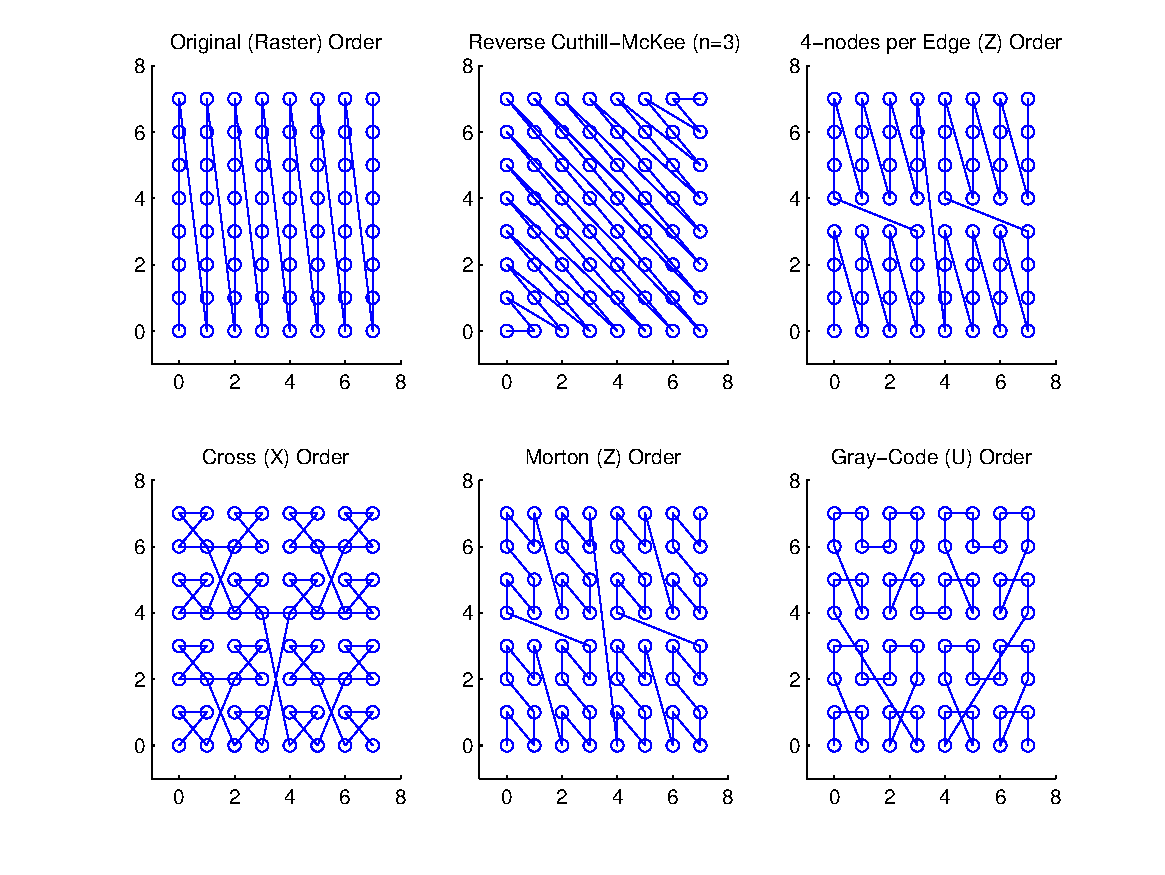
\includegraphics[width=0.65\textwidth]{rbffd_methods_content/hashing/node_orderings-eps-converted-to.pdf} \\
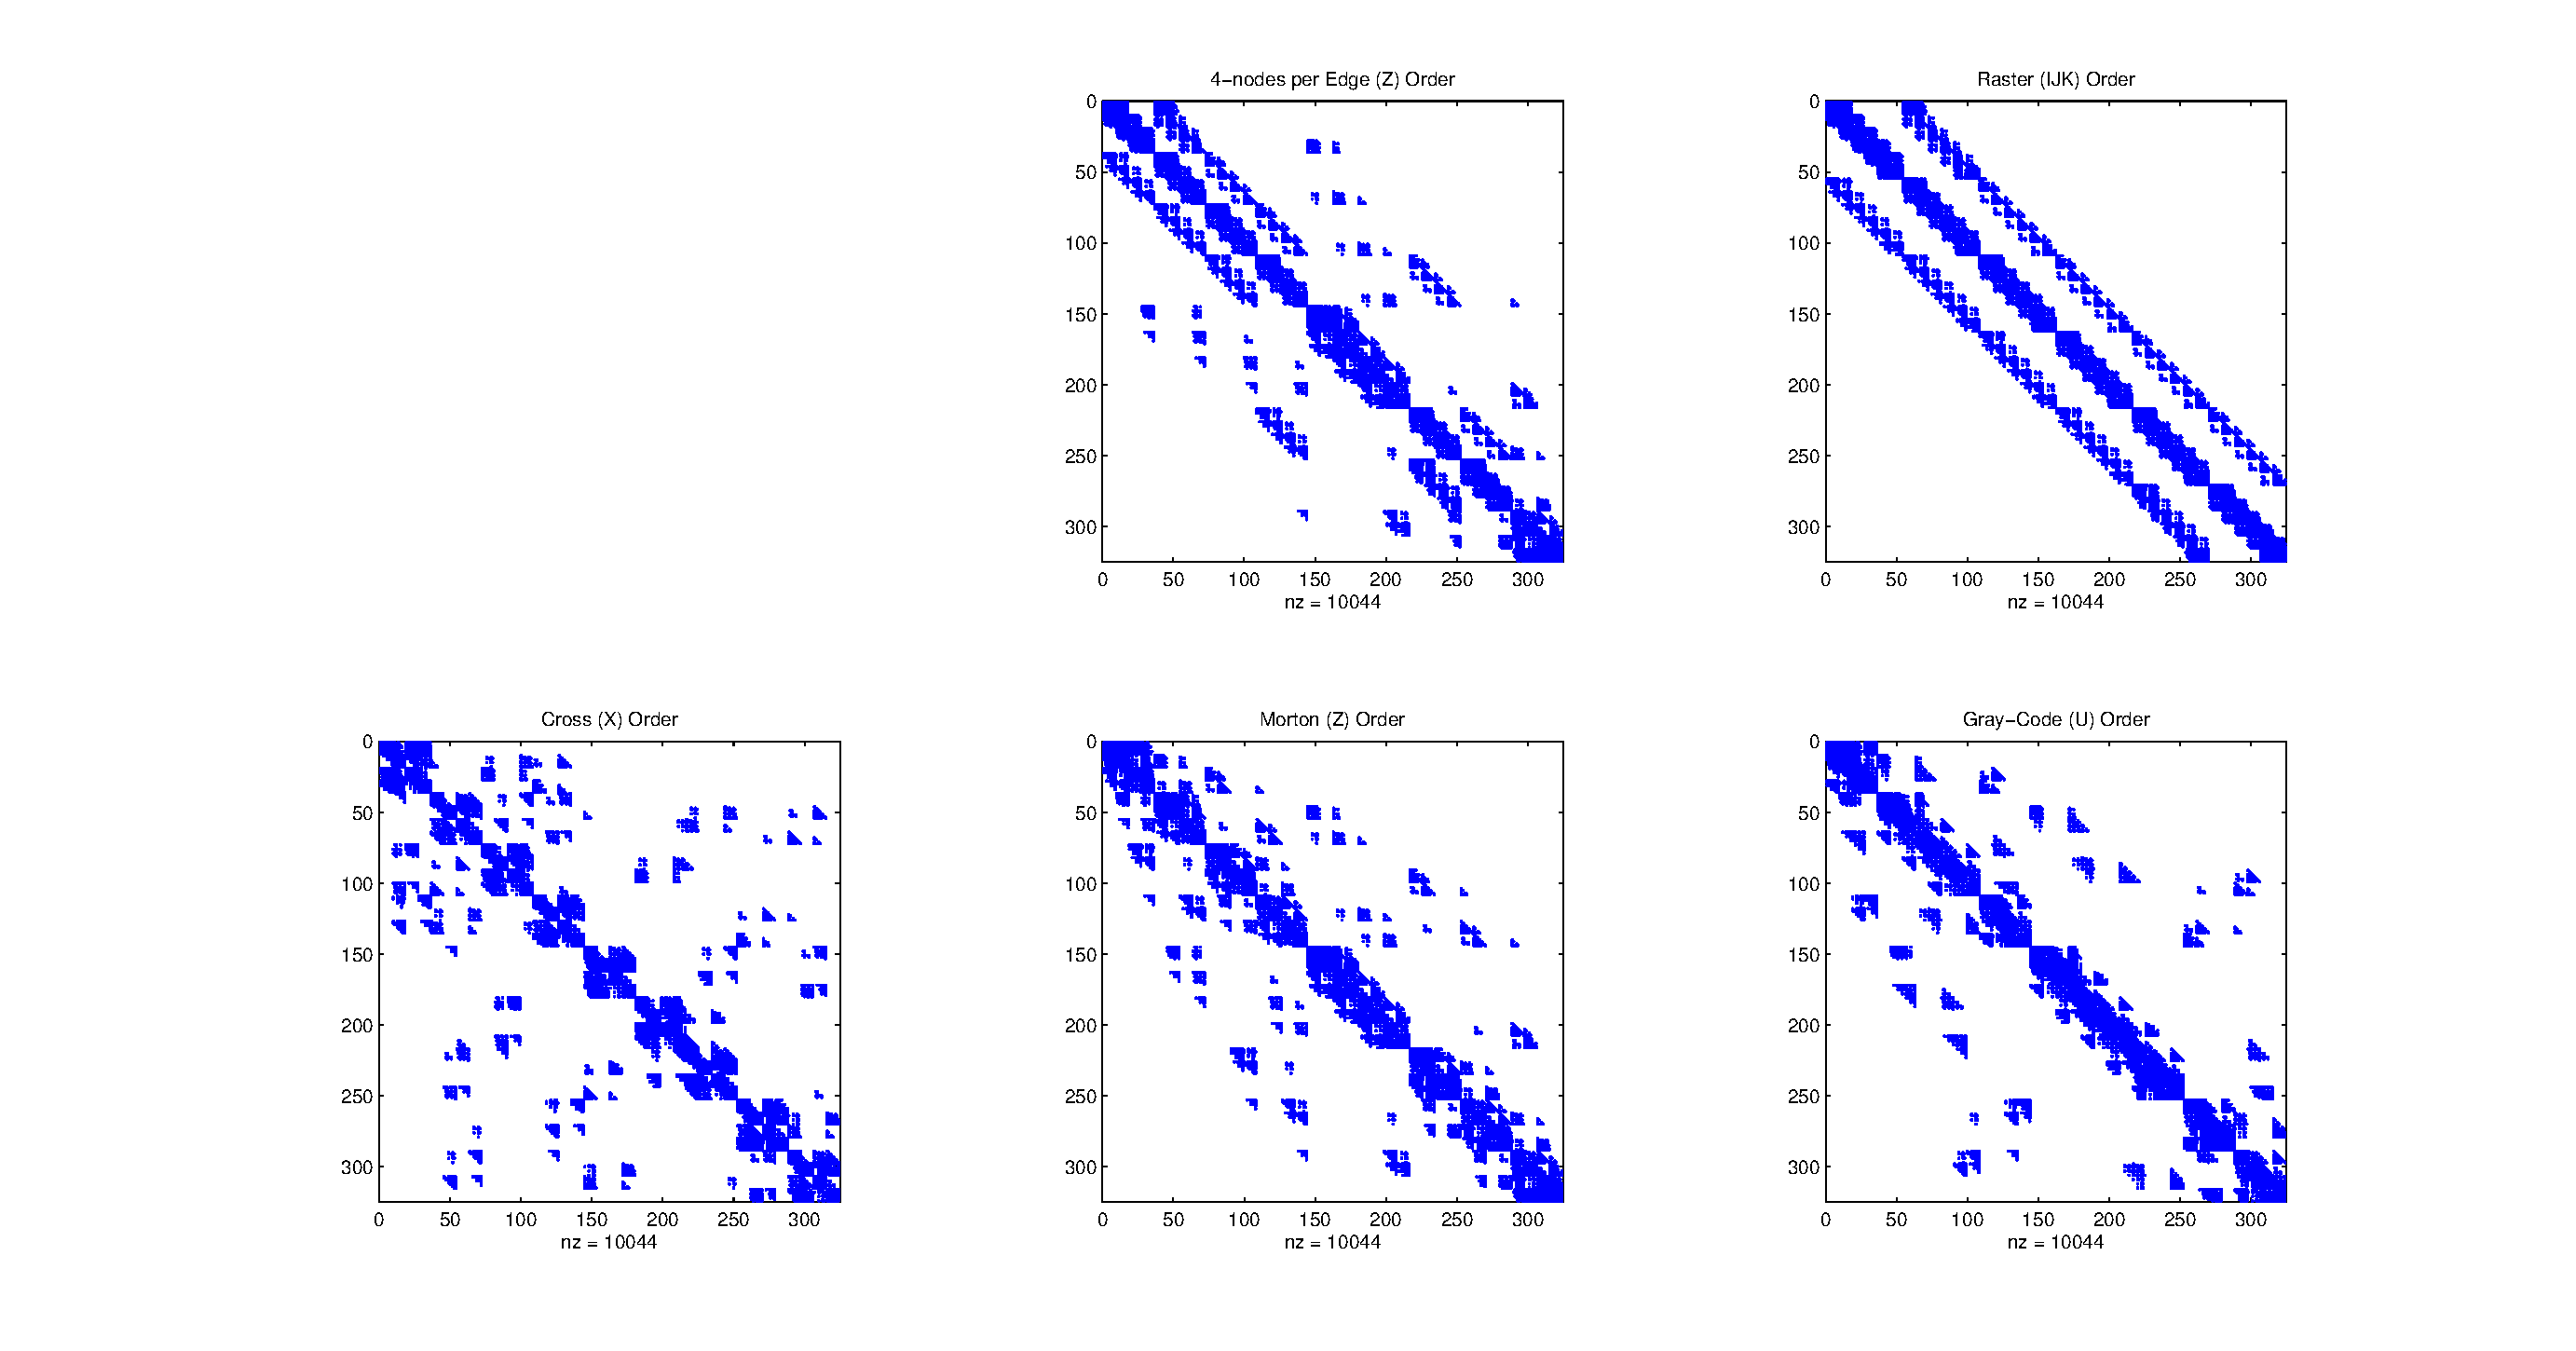
\includegraphics[width=0.65\textwidth]{rbffd_methods_content/hashing/spy_regulargrid-eps-converted-to.pdf} 
\caption{In order: a) node ordering test cases; b) original ordering of regular grid (raster); c) coarse grid overlay for hash functions ($hnx = 6$); d) example stencil ($n=31$) spanning multiple Z's; e) spy of DM after orderings. }
\label{fig:orderings}
\end{figure}


\section{Conclusions on Stencil Generation}



\ifstandalone
\bibliographystyle{plain}
\bibliography{merged_references}
\end{document}
\else
\expandafter\endinput
\fi